\documentclass[%
    corpo=12pt,
    twoside,
    oldstyle,
    tipotesi=magistrale,
    greek,
    evenboxes,
]{toptesi}

\usepackage[utf8]{inputenc}  % codifica d'entrata
\usepackage[T1]{fontenc}     % codifica dei font
\usepackage{lmodern}         % scelta dei font
\usepackage{hyperref}
\usepackage{dirtree}
\usepackage{listings}
\usepackage{csquotes}
\usepackage{array}
\usepackage{tabularx}

\usepackage{color}
\usepackage[pdftex]{xcolor}
\usepackage{textcomp}
\usepackage{caption}

\definecolor{lightgray}{rgb}{.9,.9,.9}
\definecolor{keywords}{HTML}{CC7832}
\definecolor{string}{HTML}{6A8759}
\definecolor{number}{HTML}{6897BB}
\definecolor{comment}{HTML}{2f2f2f}

% Base styling
\lstset{%
    frame=single,
    captionpos=b,
    basicstyle=\normalfont\ttfamily,
    backgroundcolor=\color{lightgray},
    extendedchars=true,
    numbers=left,
    numberstyle=\footnotesize,
    numbersep=9pt,
    tabsize=2,
    keywordstyle=\color{keywords}\bfseries,
    ndkeywordstyle=\color{keywords}\bfseries,
    identifierstyle=\color{black},
    commentstyle=\color{comment}\ttfamily,
    stringstyle=\color{string}\ttfamily,
    showstringspaces=false,
    showspaces=false,
    breaklines=true,
    showtabs=false,
}

\lstdefinelanguage{ts}{
  keywords={
    typeof, new, true, false, catch, function, return, null, catch, switch, var, if, in, while, do, else, case, break,
    interface,arguments,await, async,break,case,catch,class,const,continue,debugger,default,delete,do,else,enum,eval,export,extends,false,
    finally,for,function,if,implements,import,in,instanceof,interface,let,new,null,package,private,protected,public,return,static,super,
    switch,this,throw,true,try,typeof,var,void,while,with,yield, require, module, exports
  },
  ndkeywords={class, export, boolean, throw, implements, import, this},
  sensitive=false,
  comment=[l]{//},
  morecomment=[s]{/*}{*/},
  morestring=[b]',
  morestring=[b]",
}

\lstdefinelanguage{json}{
  keywords={true, false},
  literate=
   {:}{{{\color{comment}{:}}}}{1}
   {,}{{{\color{comment}{,}}}}{1}
   {\{}{{{\color{comment}{\{}}}}{1}
   {\}}{{{\color{comment}{\}}}}}{1}
   {[}{{{\color{comment}{[}}}}{1}
   {]}{{{\color{comment}{]}}}}{1},
}

\lstdefinelanguage{yaml}{
}

\lstdefinelanguage{shell}{
}

% Default language
\lstset{%
    language=ts
}

\lstnewenvironment{code}[1][]{
    \noindent
    \minipage{\linewidth}
    \vspace{0.5\baselineskip}
    \lstset{#1}
} {\endminipage}

\hypersetup{%
    pdfpagemode={UseOutlines},
    bookmarksopen,
    pdfstartview={FitH},
    colorlinks,
    linkcolor={blue},
    citecolor={blue},
    urlcolor={blue}
}

\interlinea{1.5}

\hyphenation{Restlessness}

\begin{document}
    \english
    \errorcontextlines=9

    \begin{ThesisTitlePage}
    \TesiDiLaurea{Master Degree Thesis}

    \ateneo{Politecnico di Torino}

    \titolo{Development, Test and Application of a framework for cloud serverless services}
    %%%%%%% Corso degli studi
    \corsodilaurea{Ingegneria Informatica}

    \TitoloListaCandidati{Candidate}
    \candidato{Andrea \textsc{Santu}}[251579]

    %%%%%%% Relatori o supervisori
    \relatore{Dr.~Ing.~Boyang Du}
    \AdvisorName{Thesis Supervisor}

    %%%%%%% Tutore
    \tutoreaziendale{Dott.\ Magistrale Antonio Giordano}
    \NomeTutoreAziendale{Intership Tutor}

    %%%%%%% Seduta dell'esame
    \sedutadilaurea{\textsc{Academic~year} 2020-2021}

    %%%%%%% Logo della sede
    \logosede{source/images/polito}

\end{ThesisTitlePage}
    \begin{abstract}
    todo\\
    brief description of the thesis
\end{abstract}
    % \begin{acknowledgements}
    todo
\end{acknowledgements}

    \renewcommand{\baselinestretch}{1.1}\normalsize
    \allcontents
    \renewcommand{\baselinestretch}{1.5}\normalsize

    \begin{mainmatter}
        \begin{chapter}{Cloud services}
    \label{chap:cloud_services}

    In the early days of the web, anyone who wanted to build a web application had
    to buy and maintain the physical hardware required to run a server, which was
    a cumbersome process to undertake, especially for small businesses
    \cite{what_is_sls_cloudflare}.
    Then came a new paradigm for the provisioning of computing infrastructure, named
    Cloud Computing, and defined as:

    \enquote*{%
        Clouds are a large pool of easily usable and accessible virtualized resources
        (such as hardware, development platforms and/or services). These resources
        can be dynamically reconfigured to adjust to a variable load (scale), allowing
        also for an optimum resource utilization. This pool of resources is typically
        exploited by a pay-per-use model in which guarantees are offered by the
        Infrastructure Provider by means of customized SLAs.%
    } \cite{cloud_computing_definition}

    \begin{figure}
        \centering
        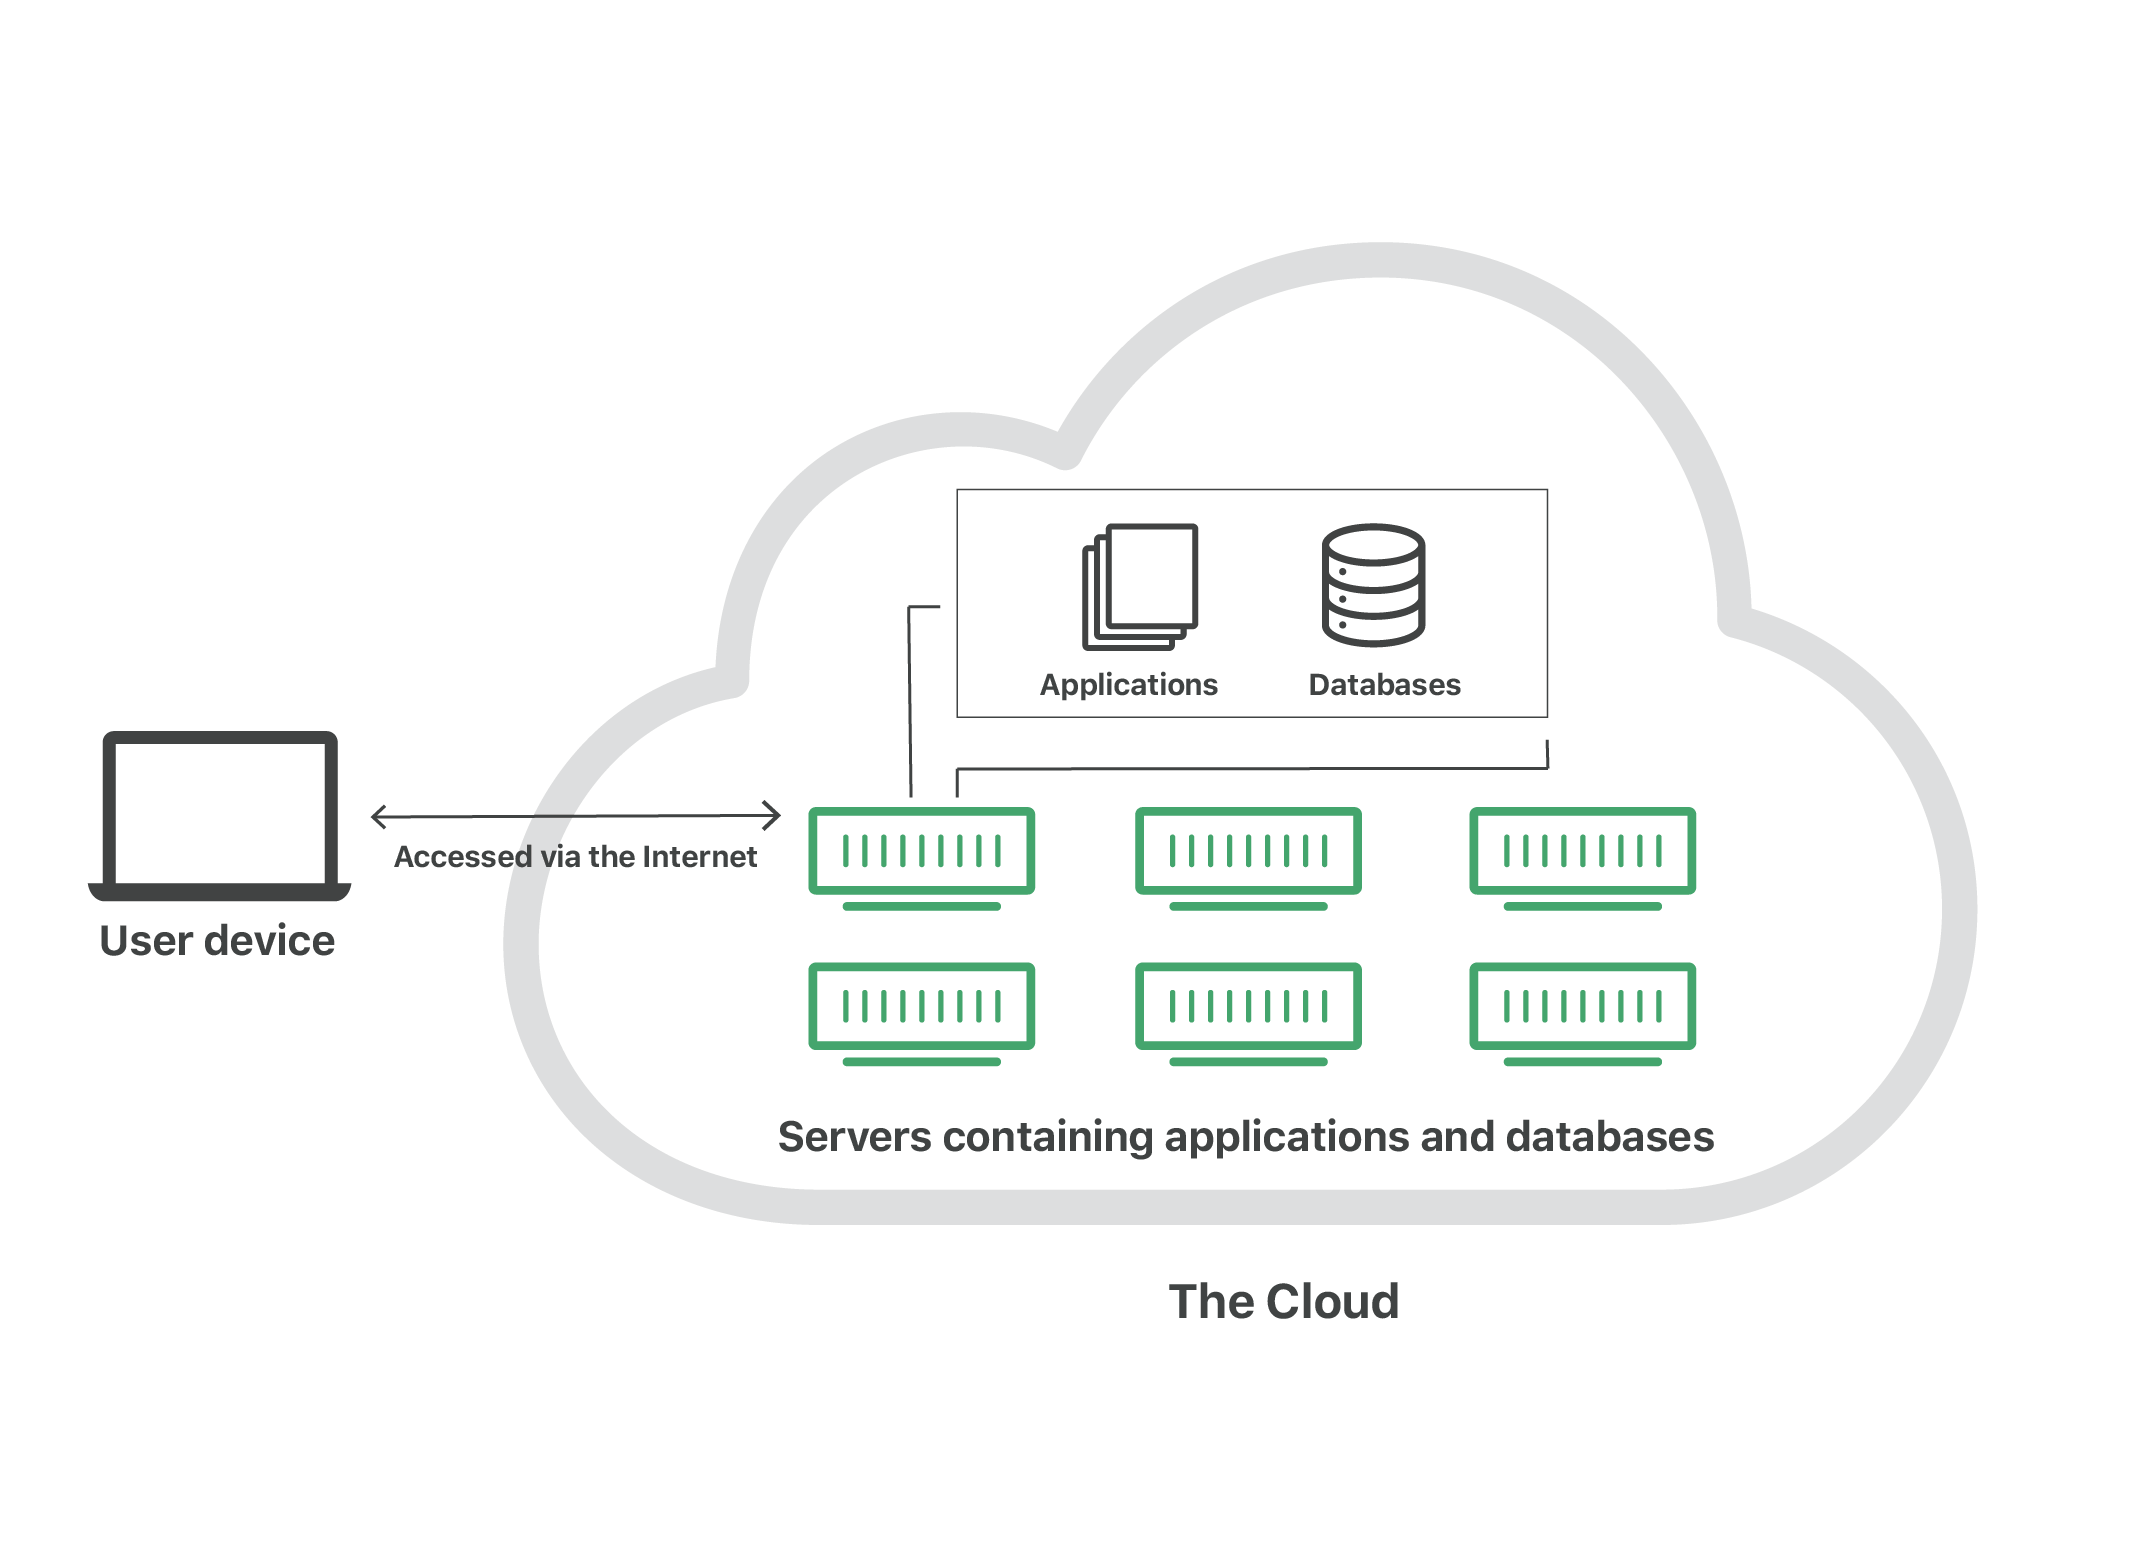
\includegraphics[width=10cm]{source/images/what-is-the-cloud.png}
        \caption{Representation of the cloud}
    \end{figure}

    Cloud Computing is possible because of a technology called virtualization, which
    allows the creation of a simulated computer, named virtual machine, that behaves
    as if it were a physical computer with its own hardware. When properly implemented,
    this approach allows having a more efficient use of the physical hardware, as
    each computer is able to run many virtual machines at once.
    Despites the many benefits, using virtual machines still requires manual server
    administration, as each one simulate a full system, including the operating
    system and the underlying kernel.

    The next technological step has been containerization, which gave the possibility
    of packing an application and all its dependencies, such as system libraries
    and system settings into a single entity called Container. With this approach
    a single physical machine, including the kernel, is shared by a multitude of
    containers. The main advantages that containerization offers, with respect to
    virtual machines are \cite{what_is_the_cloud}:
    \begin{itemize}
        \item Portability: once the application is packed into a container it can
            be run on any host supporting that technology.
        \item Control and flexibility.
        \item Faster deploy.
        \item Less server administration.
    \end{itemize}
    With this premises about the cloud and its infrastructure is possible to outline
    the main models that have emerged in the context of cloud computing.

    \section{Cloud computing models}
    Among the various types of cloud computing architectures have emerged three
    main models, which are: Infrastructure as a Service, Platform as a Service and
    Software as a Service. Each model is characterized by an increasing level of
    abstraction regarding the underlying infrastructure.

    \begin{figure}
        \centering
        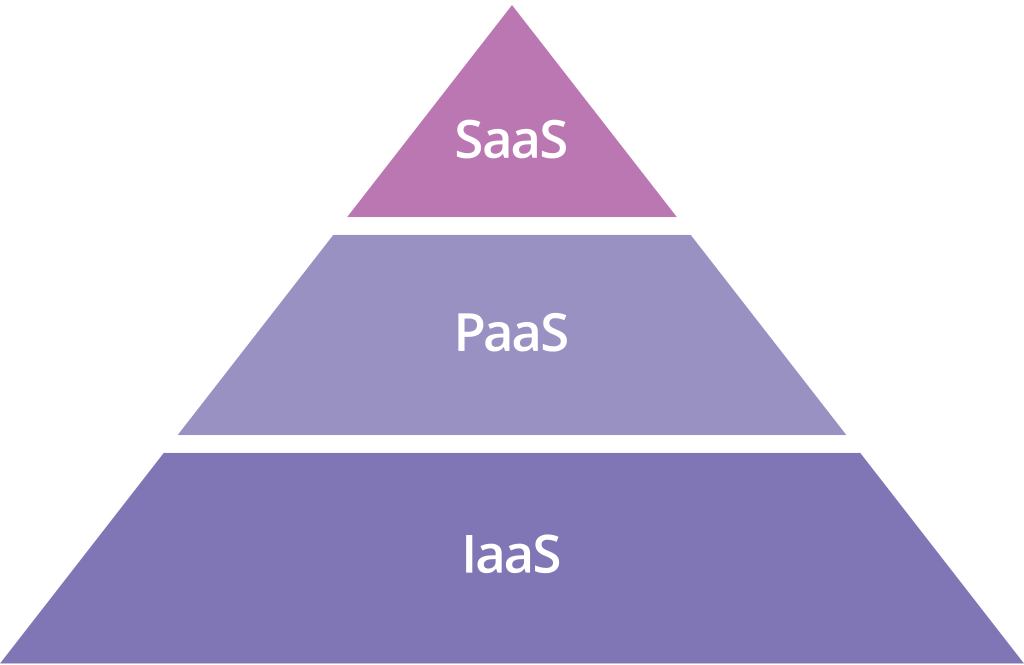
\includegraphics[height=3cm]{source/images/saas-paas-iaas-cloud-pyramid.png}
        \caption{IaaS, PaaS, SaaS Pyramid}
        \label{fig:cloud_computing_pyramid}
    \end{figure}

    \subsection{Infrastructure as a Service (IaaS)}
    Infrastructure refers to the computers and servers than run code and store data.
    A vendor hosts the infrastructure in data centers, referred to as the cloud,
    while customers access it over the Internet. This eliminates the need for customers
    to own and manage the physical infrastructure, so they can build and host web
    applications, store data or perform any kind of computing with a lot more flexibility.
    An advantage of this approach is scalability, as customers can add new servers
    on demand, every time the business needs to scale up, and the same apply also
    if the resources are not needed anymore. Essentially physical servers purchasing,
    installing, maintenance and updating operations are outsourced to the cloud
    provider, so customers can spend fewer resources on that and focus more on business
    operations, thus leading to a faster time to market. The main drawback of this
    approach is the cost effectiveness, as businesses needs to over-purchase resources
    to handle usage spikes, this leads to wasted resources \cite{iaas}.

    \subsection{Platform as a Service (PaaS)}
    This model simplify web development, from a developer perspective, as they can
    rely on the cloud provider for a series of services, which are vendor dependent.
    However some of them can be defined as core PaaS services, and those are: development
    tools, middleware, operating systems, database management, and infrastructure.
    PaaS can be accessed over any internet connection, so developers can work on
    the application from anywhere in the world and build it completely on the browser.
    This kind of simplification comes at the cost of less control over the development
    environment \cite{paas}. An example of this kind of services is Google's
    \href{https://cloud.google.com/appengine}{App Engine}.

    \smallskip
    Another model has recently been added to the three main cloud computing models,
    named Backend as a Service (Baas). This model stands, with some differences,
    at the same level of PaaS, and it's suited especially for web and mobile backend
    development. As with PaaS, BaaS also makes the underlying server infrastructure
    transparent from the developer point of view, and also provides the latter with
    api and sdk that allow the integration of the required backend functionalities.
    The main functionalities already implemented by BaaS are: database management,
    cloud storage, user authentication, push notifications, remote updating and hosting.
    Thanks to these functionalities there may be a greater focus on frontend or mobile
    development.
    In conclusion BaaS provides more functionalities with respect to the PaaS model,
    while the latter provides more flexibility.

    \subsection{Software as a Service (SaaS)}
    In this model the abstraction from the underlying infrastructure is maximized.
    The vendor makes available a fully built cloud application to customers, through
    a subscription contract, so rather than purchasing the resource once there is
    a periodic fee. The main advantages of this model are: access from anywhere,
    no need for updates or installations, scalability, as it's managed by the SaaS
    provider, cost savings.
    However there are also main disadvantages, that makes this solution not suitable
    in some cases: developers have no control over the vendor software, the business
    may become dependent on the SaaS provider (vendor lock-in), no direct control
    over security, this may be an issue especially for large companies \cite{saas}.

    \begin{figure}
        \centering
        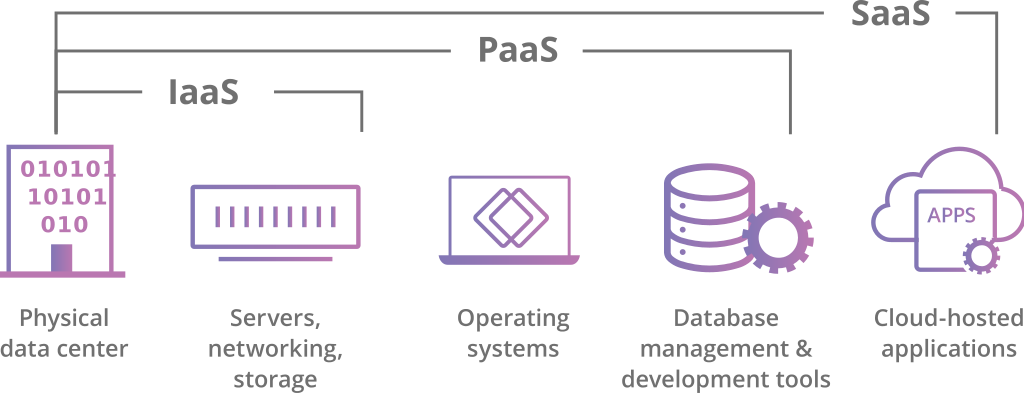
\includegraphics[width=\linewidth]{source/images/saas-paas-iaas-diagram.png}
        \caption{IaaS, PaaS, SaaS diagram}
        \label{fig:cloud_computing_architectures}
    \end{figure}

    \section{Serverless paradigm}
    The downsides of the previously described approaches varies from the control on the
    infrastructure and on the software, to scalability problems, to end with cost
    and resources utilization effectiveness.
    Aiming to solve these problems, the major providers started investing on a new
    cloud computing model, named Function as a Service (FaaS) and based on the
    serverless paradigm.
    Such a paradigm is based on providing backend services on an as-used basis, with
    the cloud provider allowing to develop and deploy small piece of code without
    the developer having to deal with the underlying infrastructure.
    So despite the terminology, serverless does not mean without servers, as they are
    of course still required, but they are transparent to developers, which can focus
    on smaller pieces of code.
    With this model, rather than over purchase the resources, to ensure correct
    functionality in all workload situations, as happens in the IaaS model, the vendor
    charges for the actual usage, as the service is auto-scaling. Thanks to this approach
    consumer costs will be fine grained as shown in \ref{fig:serverless_benefits}.

    \begin{figure}
        \centering
        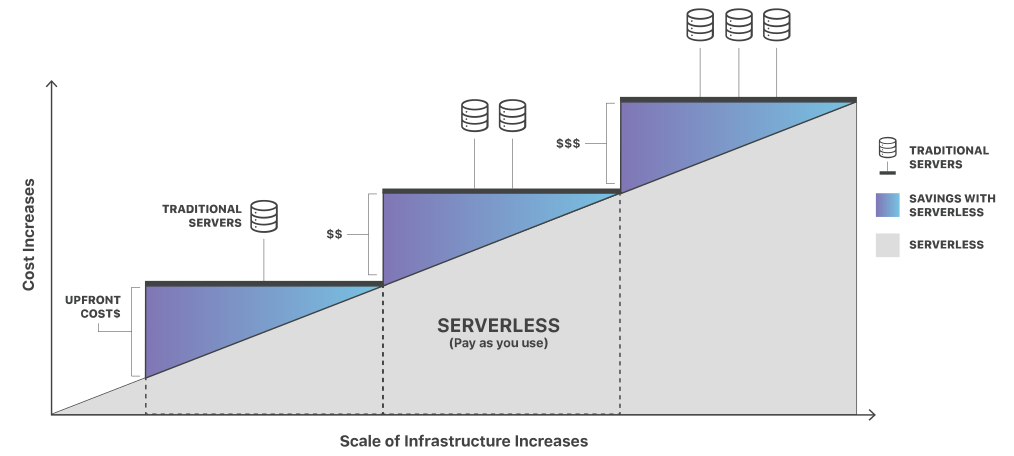
\includegraphics[width=\linewidth]{source/images/benefits-of-serverless.png}
        \caption{Cost Benefits of Serverless}
        \label{fig:serverless_benefits}
    \end{figure}

    Being the underlying infrastructure transparent for the developer, you get the advantage
    of a simpler software development process, and this advantage characterize also
    the PaaS model. Furthermore, being the service auto-scaling, is possible to obtain
    a virtually unlimited scaling capacity, as it happens in the IaaS model, where the
    limit is the cloud provider availability.

    An implementation of the serverless paradigm is the cloud model named Function
    as a Service (FaaS), which allows developers to write and update pieces of code
    on the fly, typically a single function.
    Such code is then executed in response to an event, usually an api call, but other
    options are possible, so it executed regardless of the events, and this lead to
    the previously described benefit regarding scalability and cost effectiveness.
    Furthermore, through this model turns out to be more efficient to implement web
    applications using the modular approach of the micro services architecture
    (\ref{fig:monolithic_to_microservices}), since the code is organized as a set of
    independent functions from the beginning.

    \begin{figure}
        \centering
        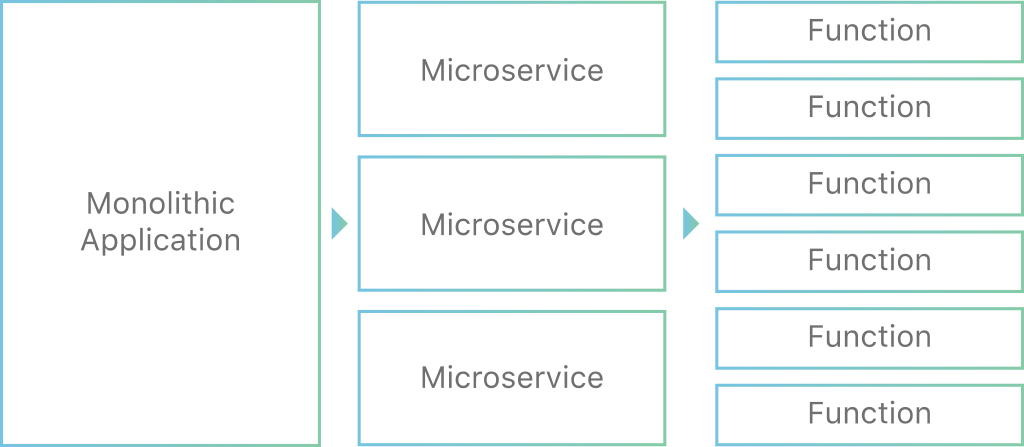
\includegraphics[width=\linewidth]{source/images/monolithic-application-microservice-faas.png}
        \caption{Monolithic to Micro services application}
        \label{fig:monolithic_to_microservices}
    \end{figure}

    So the main advantages of the FaaS model are: improved developer speed, built-in
    scalability and cost efficiency. As each approach, there are also drawbacks, in
    this case developers have less control on the system, and an increased complexity when it
    comes to test the application in a local environment.

    The first cloud provider to move into the FaaS director has been Amazon, with the
    introduction of aws lambda in 2014, followed by microsoft and google, with
    azure function and cloud function respectively in 2016.

    \section{Serverless Framework}
    \label{sec:serverless_framework}
    Shortly after the release of the service Aws lambda functions, has been introduced,
    in 2015, the Serverless framework, with the main objective of making development,
    deploy and troubleshoot serverless applications with the least possible overhead.
    The framework consists of an open source Command Line Interface and a hosted
    dashboard, that combined provide developers with serverless application lifecycle
    management. Serverless supports all runtime provided by Aws, corresponding to
    the most popular programming languages such as: Node.js, Python, Ruby, Java,
    Go, .Net, and others are on development.

    Although the serverless framework, given the number of cloud providers supported,
    aim to be platform agnostic, the following examples will be based on the Aws
    provider and on the Node.js programming language.

    The main work units of the framework, according to the FaaS model, are the functions.
    Each function is responsible for a single job, and although is possible to perform
    multiple tasks using a single function, it's not recommended as stated by the
    design principle Separation of concerns \cite{separation_of_concerns}.
    Each function is executed only when triggered by and Event, which can be of different
    type, such as: http api request, scheduled execution and image or file upload.
    Once the developer has defined the function and the events associated to it,
    the framework take care of creating the necessary resources on the provider platform.

    The framework introduces the concept of Services as unit of organization. Each
    service has one or more functions associated to it and an application can then
    be composed by multiple services. This structure reflects the modular approach
    of the micro services architecture described previously. Finally various applications
    are grouped under an organization (\ref{fig:sls_resource_scheme})

    \begin{figure}
        \centering
        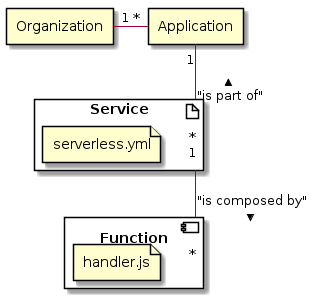
\includegraphics[width=6.5cm]{source/diagrams/serverless_app_service.png}
        \caption{Serverless framework resources scheme}
        \label{fig:sls_resource_scheme}
    \end{figure}

    A service is described by a file, located at the root directory of the project,
    and composed in the format \href{https://yaml.org/}{Yaml} or Json.
    Below is a simple serverless.yml file (listing \ref{lst:simple_sls_yml}), it
    defines the service users, which contains just a function, responsible of creating
    a user. The handler field specify the path to the function code, in this case
    the framework will search for a handler.js file, exporting a usersCreate function,
    as show on listing \ref{lst:handler_fun}.

    \bigskip
    \begin{lstlisting}[caption=Simple serverless.yml file, label={lst:simple_sls_yml}]
org: my-company-org
app: chat-app
service: users
provider:
    name: aws
    runtime: nodejs12.x
functions:
    usersCreate:
        handler: handler.usersCreate
        events:
            - http: post users/create
    \end{lstlisting}

    \begin{lstlisting}[caption=Simple handler function, label={lst:handler_fun}]
async function usersCreate(event, context) {
    const user = {
        name: 'sample_name',
        surname: 'sample_surname'
    }
    await mockDb.createUser(user)
    return {
        statusCode: 200,
        body: JSON.stringify({user})
    }
}
    \end{lstlisting}

    \begin{figure}
        \caption{Simple Serverless project structure}
        \label{fig:sls_project_structure}
        \begin{minipage}{\linewidth}
            \dirtree{%
                .1 ./.
                .2 handler.js.
                .2 serverless.yml.
            }
        \end{minipage}
    \end{figure}

    Serverless is flexible and does not force a fixed structure of the project, that
    task is up to the developer.
    Defined that structure, the service can be deployed using the Serverless CLI, on
    the chosen provider, as shown on listing \ref{lst:sls_deploy}.

    \bigskip
    \begin{lstlisting}[caption=Deploy command, label={lst:sls_deploy}]
$ serverless deploy
Serverless: Stack update finished...
Service Information
service: users
stage: dev
region: us-east-1
stack: users-dev
resources: 12
api keys:
  None
endpoints:
  POST - https://.../dev/users/create
functions:
  usersCreate: users-dev-usersCreate
layers:
  None
    \end{lstlisting}

    The deploy command creates the necessary aws resources, in this case they are:
    a lambda function corresponding to the usersCreate function and an api gateway to
    handle http requests.
    It is then possible to test the newly created resource by making requests to the
    url returned by the CLI, specifying the resource path /users/create.
    It is possible to invoke online functions also directly from the CLI,
    specifying the identifier of the function used in the serverless.yml file, as shown
    on listing \ref{lst:sls_invoke}

    \bigskip
    \begin{lstlisting}[caption=Invoke command, label={lst:sls_invoke}]
$ serverless invoke -f usersCreate
{
    "statusCode": 200,
    "body": "{\"user\":{\"name\":\"sample_name\", ...}}"
}
    \end{lstlisting}

    The development and deploy process shown for a service with a single function
    remains the same as the service complexity grows, in particular it is possible to
    modify and deploy a single function at a time, since each function has its own
    resource associated.
    This process gets along with the previously described micro services architecture.

    \subsection{Advantages}
    The main advantages of using the Serverless framework are:
    \begin{itemize}
        \item Provider agnostic: the framework aims to be independent from the chosen
            cloud provider, thus avoiding vendor lock-in. In practice this feature is
            not achieved completely, as the configuration file serverless.yml may be
            different across providers. However the main structure remains the same,
            and that simplify providers migration.
        \item Simplified development: the CLI commands simplify the development process,
            from the deploy from the testing of the deployed functions.
        \item Extensible: is possible to develop plugins that integrate with the
            CLI commands lifecycle, increasing their functionalities.
        \item Dashboard: the hosted dashboard allow monitoring and tracing of the
            deployed functions and services.
    \end{itemize}

    \subsection{Disadvantages}
    \label{subsec:sls_disadvantage}
    The main advantages of using the Serverless framework and the Serverless paradigm are:
    \begin{itemize}
        \item Compilation of the configuration file may become tedious as the project grows.
        \item The framework is extremely flexible regarding the project structure and
            that is an advantage, however this can be also a drawback as it's up to the
            developer to find a suitable structure, and this means less time spent on
            business related tasks.
        \item Unit testing: it is possible to test a deployed function easily, however
            for big projects, where it's necessary to test a lot of functions, this may
            become cumbersome.
        \item Resource threshold: for projects created with Aws, a single
            serverless.yml file may create up to 200 resources, and if exceeded
            the deploy operation fails. Since each function is responsible for the
            creation of about 10 resources, is very easy to exceed this limit.
            The only solution so solve this problem is to split the functions across
            multiple services, hence different serverless.yml configuration files.
        \item Cold start: inherent overhead of the current implementation of the
            serverless paradigm. Since each function is executed only in response to
            an event, a certain amount of time is required for resources initialization.
    \end{itemize}

    \section{Conclusions}
    Each cloud model presented has its own strength and drawbacks, depending on the
    needs of the wanted goal. Favouring as selection criteria, solutions that present
    major advantages in terms of scalability, cost efficiency and speed of development,
    has been decided to favour the Serverless option.
    The main cloud providers offering this kind of service, as previously stated,
    are: Aws, with its Lambda service, Microsoft, with Azure Functions, and Google,
    with Cloud Functions. Each provider offer different configurations, with different
    pricing, based on memory, CPU, and execution time as parameters, as shown on
    \ref{table:cloud_providers_offer}.
    In the literature there are several documents comparing the various services
    side by side exhaustively \cite{sls_providers_comparison}.
    For the project subject of this document has been chosen Aws as the main provider,
    as the most mature platform meeting the project's needs. In particular it
    providers the following advantages with respect to the competitors \cite{sls_providers_comparison}:
    \begin{itemize}
        \item Cold start (\ref{table:cloud_providers_cold_start})
        \item Overall maturity
        \item Performance consistency
        \item Scalability
    \end{itemize}

    \begin{table}
        \centering
        \begin{tabularx}{0.8\textwidth}{
                | >{\raggedright\arraybackslash}X
                | >{\centering\arraybackslash}X
                | >{\centering\arraybackslash}X
                | >{\centering\arraybackslash}X |
            }

            \hline
            & \textbf{AWS} & \textbf{Azure} & \textbf{Google} \\
            \hline\hline
            Memory (MB) & 64 * k (k = 2, 3, ..., 24) & 1536 & 128 * k (k = 1, 2, 4, 8, 16) \\
            \hline
            CPU & Proportional to Memory & Unknown & Proportional to Memory \\
            \hline
            Language & Python Nodejs Java, and others & Nodejs Python, and others & Nodejs \\
            \hline
            Runtime OS & Amazon Linux & Windows 10 & Debian 8 \\
            \hline
            Local disk (MB) & 512 & 500 & > 512 \\
            \hline
            Run native code & Yes & Yes & Yes \\
            \hline
            Timeout (second) & 300 & 600 & 540 \\
            \hline
            Billing factor & Execution time, Allocated memory & Execution time,
                Consumed memory & Execution time, Allocated memory, Allocated CPU\\
            \hline
        \end{tabularx}
        \caption{Cloud providers configuration \cite{sls_providers_comparison}}
        \label{table:cloud_providers_offer}
    \end{table}

    \begin{table}
        \centering
        \begin{tabularx}{0.8\textwidth}{
                | >{\raggedright\arraybackslash}X
                | >{\centering\arraybackslash}X
                | >{\centering\arraybackslash}X
                | >{\centering\arraybackslash}X
                | >{\centering\arraybackslash}X |
            }

            \hline
            Provider-Memory & Median & Min & Max & STD \\
            \hline\hline
            AWS-128 & 265.21 & 189.87 & 7048.42 & 354.43 \\
            \hline
            AWS-1536 & 250.07 & 187.97 & 5368.31 & 273.63 \\
            \hline
            Google-128 & 493.04 & 268.5 & 2803.8 & 345.8 \\
            \hline
            Google-2048 & 110.77 & 52.66 & 1407.76 & 124.3 \\
            \hline
            Azure & 3640.02 & 431.58 & 45772.06 & 5110.12 \\
            \hline
        \end{tabularx}
        \caption{Cloud providers Cold start (in ms) \cite{sls_providers_comparison}}
        \label{table:cloud_providers_cold_start}
    \end{table}

\end{chapter}
        \begin{chapter}{Tools}

    An important process in the software development is the choice of the right
    tools, in order to achieve simplicity and efficiency for both development
    process and the project itself.
    In this chapter will be described the main tools used during the development
    of Restlessness and its deployment to make it available for everyone.

    \section{JavaScript}
    JavaScript is a lightweight interpreted programming language. Interpreted means
    that the code is read top to bottom, and the result of the running code is
    immediately returned. Interpreted programming languages are opposed to compiled
    one, where the code is transformed into a binary format that can be directly
    executed \cite{what_is_js}.
    Although JavaScript was born as a language limited to client side programming,
    exploiting an engine directly incorporated into the Web browser, with the
    introduction of Node.js has become possible to use this language also for backend
    programming, and in general in contexts outside of the browser.
    Node.js is a JavaScript runtime based on the V8 engine, core engine of the popular
    Chrome browser \cite{node_org}.
    A key characteristic and one of the main strength of JavaScript with respect
    to other programming languages is its asynchronous nature, that allows having
    non-blocking I/O. As a consequence of this, the code runs on a single thread,
    based on a LIFO queue (Last In, First Out) continuously checked by the so called
    Event Loop.
    As shown on \ref{fig:event_loop}, operations regarding File System, Network or
    Database access are executed separately, and only once completed are inserted
    again into the queue, to handle their result. Meanwhile other queued code
    is executed by the only present thread.

    \begin{figure}
        \centering
        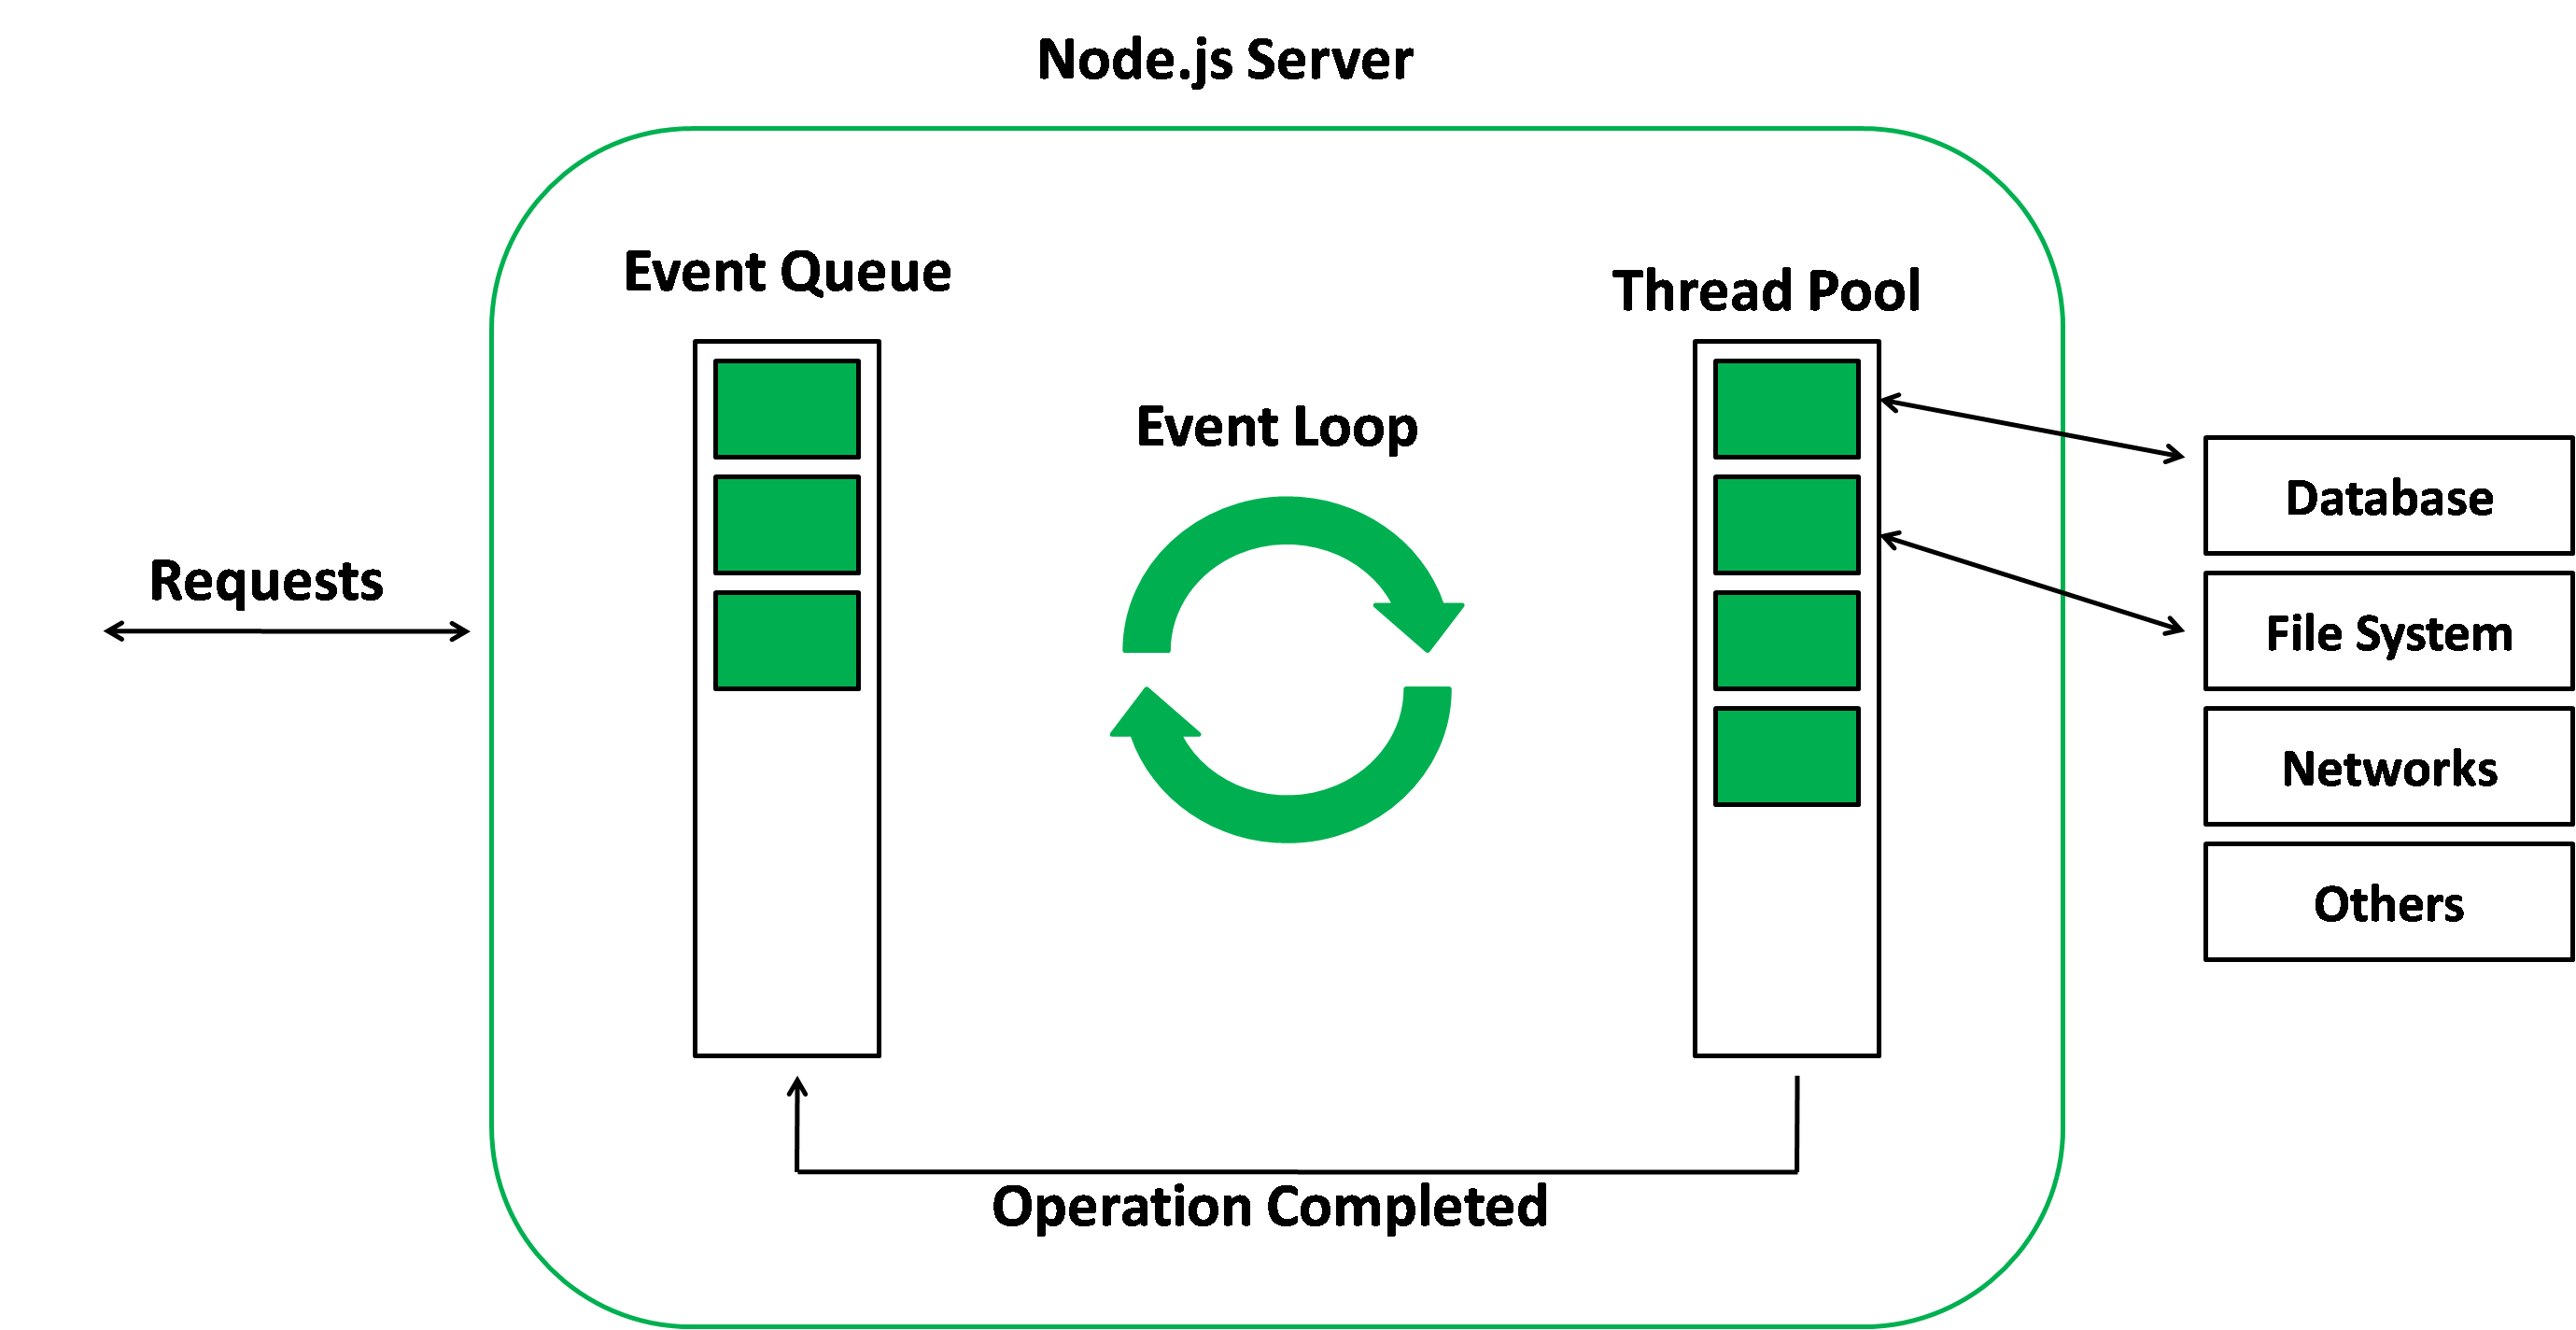
\includegraphics[width=\linewidth]{source/images/nodejs_event_loop.png}
        \caption{The Event Loop \cite{node_event_loop_2}}
        \label{fig:event_loop}
    \end{figure}

    Being single threaded is a useful limitation as it's not possible to incur
    into concurrency issues.
    This peculiarities make JavaScript well suited for the so called real-time
    applications (RTAs), that is applications that have to process a high volume
    of short messages requiring low latency, and so they require a highly scalable
    solution. Conversely due to its single threaded nature, JavaScript is not
    recommended for CPU-heavy jobs, as the Event Loop would be stuck on a single
    operation \cite{node_event_loop}\cite{node_on_backend}.

    Another advantage of JavaScript, especially after the release of Node.js, is
    the possibility to use the language for both frontend and backend in the context
    of Web development, creating a seamless experience for developers.

    JavaScript is a dynamically typed language, which means that it's not necessary
    to explicitly mention the type of data a variable holds, as that type can change
    dynamically as the content of the variable changes (\ref{lst:dynam_type}).

    \begin{code}[caption=Dynamically typed variables, label={lst:dynam_type}]
let a = "Hello World!"
a = 42
    \end{code}

    This feature of the language gives a lot of flexibility to developers, however
    as the project complexity grows it can quickly become a downside.
    For this reason, in 2012 Microsoft released an open source language called
    Typescript, a superset of JavaScript that enable static type checking.
    Being a superset, any JavaScript code is also valid Typescript code, enabling
    a gradual integration for already existing code bases.
    The Typescript compiler is specifically a transpiler, or a compiler that takes
    source code as input and produces other source code as output, in this case
    JavaScript code. The compiler will point the errors it encounters, but it does
    not prevent the code to be run, hence it behaves like a spellchecker for the code.
    Typescript can also infer variables type from their usage, reducing the effort
    needed to enable static type checking from the developer
    \cite{typescript_lang}\cite{typescript}.
    Keeping in mind the described strengths of the JavaScript environment, it has been
    decided to use it as the main language for the development of the Restlessness
    framework.

    \bigskip
    \begin{code}[caption=Static type checking on Typescript, label={ts_static}]
interface Student {
  name: string
  graduationYear: number
}

const aStudent: Student = {
  name: 'Arthur Dent',
  graduationYear: 2020
}

aStudent.graduationYear = '2020'    // Invalid
aStudent.graduationYear = 2021      // Valid
    \end{code}

    \section{Npm}
    The strengths of the JavaScript ecosystem are further increased by the presence
    of Npm, shorthand for Node Package Manager, which is the official package manager
    for Node.js. Npm rely on the CommonJs modules specification \cite{common_js},
    which defines a convention for the JavaScript module ecosystem.
    The main components of Npm are:
    \begin{itemize}
        \item Npm registry: modules can be published to it or installed from it.
            The official and main registry is available at the address
            \url{https://npmjs.org}
        \item \textit{npm} CLI: the command line tool from which is possible to interact
            with the registry, with operations like publishing or installing packages.
        \item \textit{package.json}: a configuration file, in the Json format
            \cite{jsoniso}, that must be present for both modules that are published
            into the registry and modules that use other modules from the registry
            as dependencies. It contains projects informations, such as name and
            version, and a list of other modules, on which the project depends on.
        \item \textit{node\_modules}: an automatically created folder that contains
            all the projects dependencies. At runtime Node.js looks for modules
            in this folder.
    \end{itemize}

    Listing \ref{lst:add_module} shows the \textit{package.json} of a simple module,
    while \ref{lst:add_fn} shows the definition of a function, on that module,
    exported using the CommonJs specification. To publish the package on the Npm
    registry is possible to invoke the \textit{publish} command on the \textit{npm}
    CLI. With the \textit{install} command that same package is installed as
    dependency under the \textit{node\_modules} folder, and can be used as shown
    on listing \ref{lst:add_require}

    \bigskip
    \begin{code}[caption=A simple \textit{package.json},
        label={lst:add_module}, language=json]
{
    "name": "add_module",
    "version": "1.0.0",
    "description": "Simple module example",
    "main": "index.js",
    "author": "Arthur Dent",
    "license": "ISC"
}
    \end{code}

    \bigskip
    \begin{code}[caption=CommonJs module definition, label={lst:add_fn}]
// index.js
function add(n1, n2) {
  return n1 + n2
}

module.exports = add
    \end{code}

    \bigskip
    \begin{code}[caption=CommonJs module usage, label={lst:add_require}]
const add = require('./add.js')
    \end{code}

    The Npm ecosystem has been used extensively during the development of Restlessness,
    for its dependencies and for making it available on the registry.
    Furthermore, the developed framework uses a feature of Npm called Scoped Packages
    \cite{npm_scoped_packages}, which allows to group related packages together
    under a common scope, acting as a namespace. Restlessness packages are available
    under the \textit{@restlessness/} scope.

    \section{Github}
    \subsection{Git}
    Git is an Open Source Distributed Version Control System, in particular:
    \begin{itemize}
        \item Control System: Git is a content tracker, it can be used to store
            content, which generally is code.
        \item Version: the tracked content is subject to continuous change, often
            this changes are added in parallel. Git helps handling this by maintaining
            a history of all changes.
        \item Distributed: Git is based on remote and local repositories, the first
            one stored in a server, while the latter is stored in the developer
            computer, and both contains the full history information.
    \end{itemize}

    Git is useful to track code changes in all cases, but it's absolutely necessary
    to avoid conflicts when multiple developers work in parallel on a single codebase.
    The main concepts introduced by Git are:
    \begin{itemize}
        \item Commit: the main unit representing content modification.
        \item Branches: allow working simultaneously at the codebase, making
            different modifications.
        \item Push/Pull: operations that allow synchronization between the remote
            repository and the local one.
        \item Merge: operation that integrate the modification made on a branch
            into another branch.
        \item Tag: a string identifier assigned to a specific commit, useful to
            reference a particular version of the project (e.g. a simple tag is
            \textit{v1.0.2}).
    \end{itemize}

    \begin{figure}
        \centering
        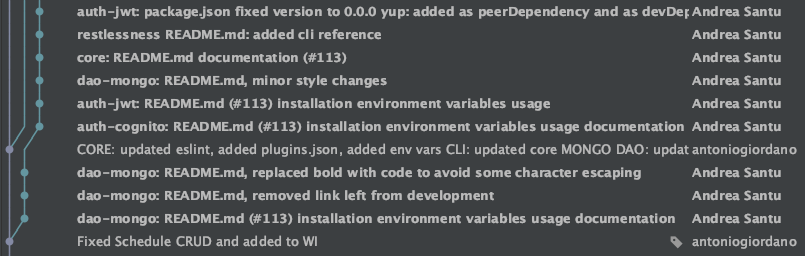
\includegraphics[width=\linewidth]{source/images/rln-git-history.png}
        \caption{Section of Restlessness history}
    \end{figure}

    With these concepts it is possible to work on each feature independently from
    others, integrating it only when it reaches an appropriate stability level.
    The strategy adopted with the developed framework has been to create branches
    with the \textit{feature/} prefix for new functionalities or improvement of
    existing ones, and the \textit{fix/} prefix for correction of bugs, followed
    by the name of the specific feature of fix.

    \subsection{Github features}
    Github is a web based platform providing all functionalities offered by the Git
    system plus additional DevOps features, with the main ones used during the
    development of Restlessness being: Issues, Pull Requests and Projects.

    \subsubsection{Issues}
    Issues are Github feature that helps to keep track of tasks, bugs, enhancements
    or any kind of modification to the project. They are characterized by a title,
    that gives an immediate feedback about what is the reason of the Issue, and an
    optional description, with more specific and technical information, as shown
    on figure \ref{fig:rln_issue}. Each Issue can be assigned to one or more
    collaborators, responsible for having it solved. This tracking system is focused
    on collaboration, as it is possible to comment and discuss about the Issue with
    other collaborators, also referencing other resources, which can be other Issues
    or code sections.
    As the project grows so does the number of Issues, and so it becomes important to
    keep them organized. This is made possible by using Labels and Milestones.
    Both allow to group Issues according to a common characteristic, but with a
    different granularity \cite{github_issues}.
    The first one allows a more specific grouping, with the main ones defined for
    Restlessness being:
    \begin{itemize}
        \item \textit{enhancement}: A new feature, or a request for a new feature.
        \item \textit{bug}: A problem in the project functionalities.
        \item \textit{documentation}: Improvements or additions to documentation.
        \item \textit{tests}: Testing related Issues
        \item \textit{good first issue}: Being the framework Open Source, also
            external people can contribute to it, this Label marks simple and easy
            Issues that can be managed also by newcomers.
        \item Packages specific Issues: Restlessness adopt a monorepo  strategy
            \cite{monorepo}, having all provided packages under the same repository,
            so it has been defined a Label for each package, such as: \textit{CORE},
            \textit{CLI}, \textit{AUTH-cognito} and \textit{DAO-mongo}.
    \end{itemize}
    The latter instead group together Issues linked together from a temporal point
    of view, typically a version release or a planned Sprint if following the agile
    methodology \cite{agile}. With the Restlessness framework it has been opted for
    the first option.


    \begin{figure}
        \centering
        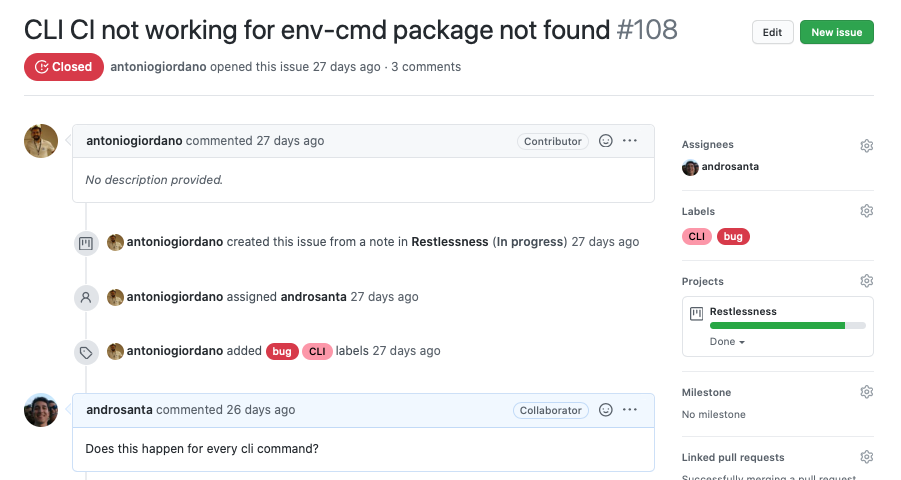
\includegraphics[width=\linewidth]{source/images/github-rln-issue.png}
        \caption{An Issue on the Restlessness project}
        \label{fig:rln_issue}
    \end{figure}

    \begin{figure}
        \centering
        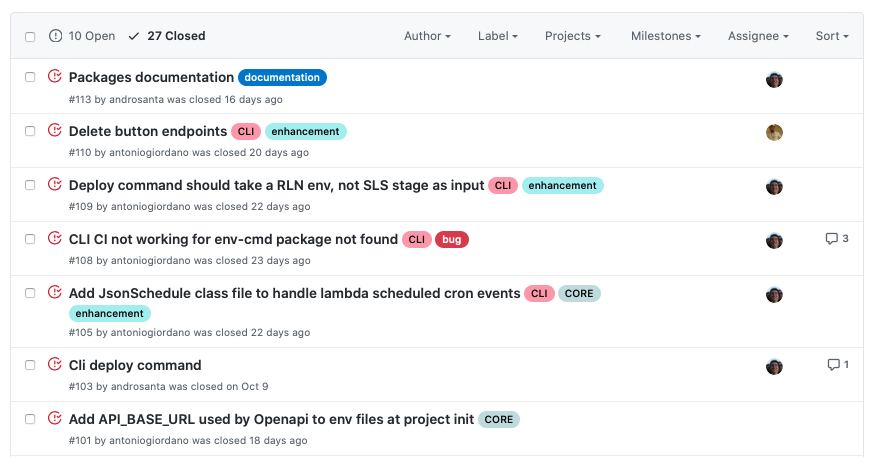
\includegraphics[width=\linewidth]{source/images/github-rln-issues-list.png}
        \caption{List of closed Restlessness Issues}
        \label{fig:rln_issues_list}
    \end{figure}

    \subsubsection{Pull Requests}
    An important process when multiple developers collaborate on a single project
    are code reviews, as having project's modification verified by more than one
    person reduces the risk of finding bugs, typos and critical problems later.
    Pull Requests are a feature of Github that enable this process. With it a
    collaborator proposes its changes while another one accepts or rejects the request.
    It is possible to discuss on the specific request, referencing other resources,
    commenting on code or requesting modification on the proposed changes, as it
    happens for Issues.
    When a Pull Request is created the author chooses a target branch on which to
    integrate its proposed changes, and once the request is accepted those changes
    are merged into the target branch, and the Pull Request is considered closed,
    as shown on figure \ref{fig:rln_pull_request}.

    \begin{figure}
        \centering
        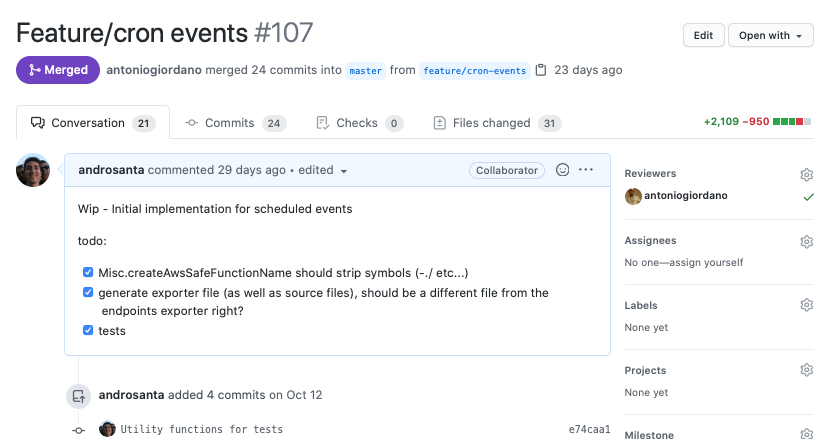
\includegraphics[width=\linewidth]{source/images/rln-pull-request.png}
        \caption{An approved Pull Request on the Restlessness project}
        \label{fig:rln_pull_request}
    \end{figure}

    \subsubsection{Projects}
    Projects is a recently added Github feature with the purpose of further improve
    organizing and distributing tasks and work. From the Projects page it is possible
    to define custom columns in which assign different tasks, which can be Issues,
    Pull Requests or simple Notes. As shown in figure \ref{fig:rln_project_board},
    for Restlessness has been defined tree columns: \textit{To do},
    \textit{In Progress} and \textit{Done}. This way it is immediately visible which
    tasks need to be done, are under development or are already completed.

    \begin{figure}
        \centering
        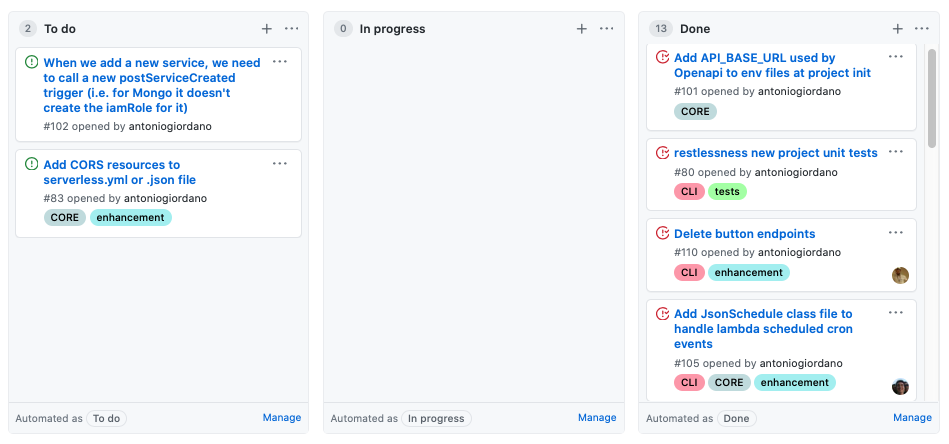
\includegraphics[width=\linewidth]{source/images/rln-github-project-board.png}
        \caption{Github Projects board on Restlessness}
        \label{fig:rln_project_board}
    \end{figure}

    \bigskip
    \bigskip
    \noindent
    Being the developed framework Open Source, it is available for consultation,
    modification and improvement on Github, as well as this document, on the
    following addresses:
    \begin{itemize}
        \item Restlessness: \url{https://www.github.com/getapper/restlessness}
        \item Thesis: \url{https://www.github.com/androsanta/Thesis}
    \end{itemize}

    \section{CircleCi}

    \subsection{CI/CD}
    Continuous Integration is a practice that encourages developers to integrate
    their code changes early and often, into the main and stable version of the
    project, which for a git based project is the \textit{master} branch.
    Each code integration triggers an automated build and test, that if failed can
    be repaired quickly.
    The main advantage of using this approach is the early bug detection, which
    as consequence will result in an overall reduced bug count and reduced
    maintenance. Moreover once set, the CI process does not add any overhead to
    the development as it is completely automated.
    The CI approach is oftentimes related to another approach, which is the
    Continuous Delivery, defined as:

    \enquote*{%
        Continuous Delivery (CD) is a software engineering approach in which teams
        keep producing valuable software in short cycles and ensure that the
        software can be reliably released at any time.%
    } \cite{continuous_delivery}

    \subsection{The platform}
    CircleCi is an online platform that provides services for implementing
    Continuous Integration and Continuous Delivery (CI/CD) on software projects.
    It can be configured to access the source code repository on Github, and after
    that each commit can trigger an automated build, test and deploy task.
    Those automated tasks are performed inside a clean container or Virtual Machine,
    ensuring a reproducible environment.

    \begin{figure}
        \centering
        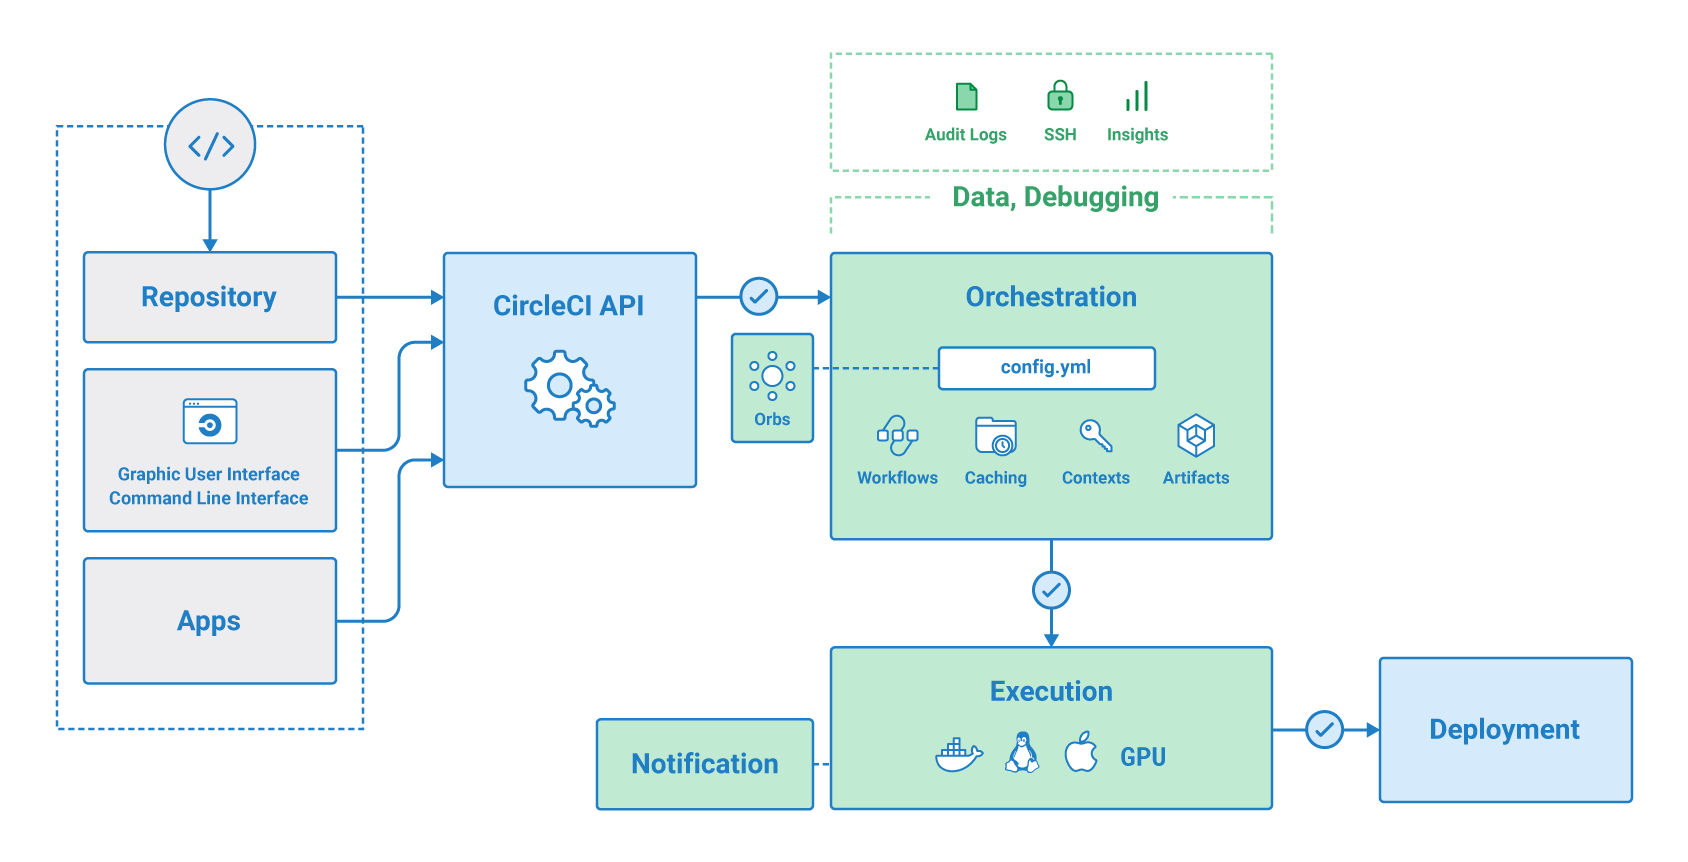
\includegraphics[width=\linewidth]{source/images/circle-ci.png}
        \caption{CircleCi flow \cite{circle_ci_official}}
        \label{fig:circle_ci_structure}
    \end{figure}

    \noindent
    The main concepts introduced by the platform are:
    \begin{itemize}
        \item Configuration: All processes are orchestrated through a single file
            called \mbox{\textit{config.yml}}, in the \href{https://yaml.org/}{Yaml}
            format, and placed under a folder called \textit{.circleci} at the root
            of the project.
        \item Orbs: Reusable snippets of code that help automate repeated processes
        \item Jobs: Building blocks of the configuration file, they are a collection
            of steps, which run commands or scripts as specified. Each Job is run
            in a unique executor.
        \item Executor: The container or Virtual Machine that run each Job.
            It is possible to chose between \href{https://www.docker.com/}{Docker}
            containers, Virtual Machines running Linux, Windows or MacOS.
        \item Steps: Actions that need to be taken to complete a Job. It can be
            any kind of executable command.
        \item Workflows: They define a list of Jobs with their run order, and
            concurrency.
    \end{itemize}

    For the Restlessness development has been chosen the popular containerization
    solution called \href{https://www.docker.com/}{Docker}, in particular a Node.js
    based container, as shown on listing \ref{lst:ci_executor}:

    \bigskip
    \begin{code}[caption=Reusable executor definition, label={lst:ci_executor},
        language=yaml]
executors:
  node12:
    docker:
      - image: circleci/node:12.9.1
    \end{code}

    As previously said the framework adopt a monorepo structure, so it has been
    necessary to define multiple Workflows, one for each package. Each Workflow
    defines two parallel Jobs, for testing and publishing on the Npm registry.
    Figure \ref{fig:ci_workflow_diagram} show the described structure for two Restlessness
    packages, and it is possible to notice that each Job run in its own container,
    in parallel and independently from the others

    \begin{figure}
        \centering
        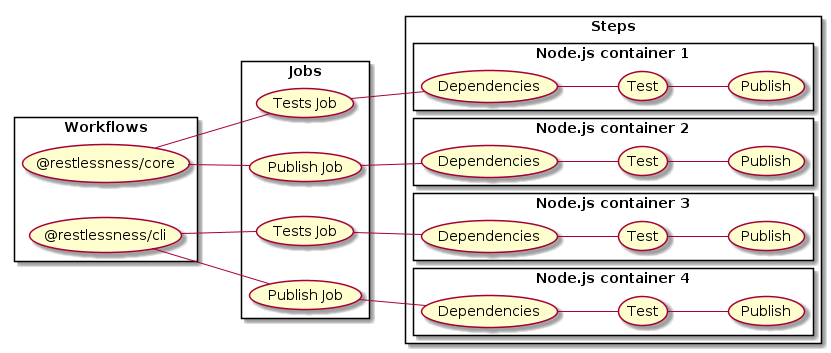
\includegraphics[width=\linewidth]{source/diagrams/ci_workflow.png}
        \caption{CircleCi workflows for Restlessness}
        \label{fig:ci_workflow_diagram}
    \end{figure}

    To perform the Steps shown on \ref{fig:ci_workflow_diagram} has been defined
    reusable commands, with the main one being:
    \begin{itemize}
        \item \textit{install\_packages}: Install dependencies as specified by the
            \textit{package.json}.
        \item \textit{deps\_and\_tests}: Install dependencies and run tests as
            specified by the \mbox{\textit{package.json}}.
        \item \textit{npm\_publish}: Publish the package on the Npm registry.
    \end{itemize}

    According to the Continuous Delivery approach the publish operation is triggered
    manually by performing a git tag on a specific repository commit, following the
    format: package name, followed by \textit{/v} and the semantic version of the
    package (e.g. \textit{@restlessness/core/v1.0.2}). A custom script takes care
    of extracting the version information and setting it on the correct
    \textit{package.json}, where is read from the npm publish command.

    Although CircleCi offers its own website from which is possible to check Workflows
    execution, errors and details of every operation, it offers also a Github plugin,
    that is able to show Workflows result directly on commits or Pull Requests, as
    shown on \ref{fig:ci_github_integration}. The integration between the two
    services has simplified the development workflow of Restlessness, and it adds to
    the already described advantages of adopting a CI/CD approach.



    \begin{figure}
        \centering
        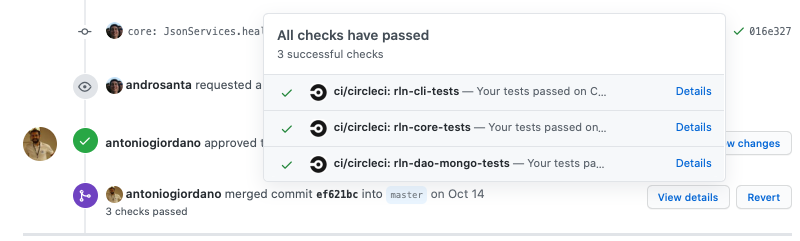
\includegraphics[width=\linewidth]{source/images/ci-github-integration.png}
        \caption{CircleCi Workflows seen from Github}
        \label{fig:ci_github_integration}
    \end{figure}

    \section{AWS}
    Amazon Web Services is a cloud platform offered by \textit{Amazon.com, Inc}
    which, among its various services, also provides serverless computing options.
    Although one of the purpose of using the Serverless Framework is to abstract
    the underlying infrastructure details of the platform, those details are needed
    to develop a framework such as Restlessness, that has to interact with the
    platform at a lower level to provide its functionalities.

    Here is a list of the main services used by Serverless and Restlessness on
    behalf of the user and also used during Restlessness development:
    \begin{itemize}
        \item Lambda: The compute service providing the serverless functionalities.
            A Lambda function contains the code written by the developer.
        \item API Gateway: A service that creates a connection point between
            external requests and other internal services, such as a Lambda functions.
        \item S3: Acronym for Simple Storage Service, provides object storage.
            Resources are organized in containers called Buckets.
        \item CloudFormation: A service that allow to model infrastructure as code.
            Each CloudFormation configuration corresponds to a resource called
            CloudFormation Stack, containing the description of other resources,
            such as AWS Lambda functions, API Gateway, and how such resources may
            interact.
        \item CloudWatch: A services for monitoring and observability.
        \item IAM:Acronym for Identity and Access Management, enables the management
            of AWS resources access.
    \end{itemize}

    \subsubsection{Resource creation during deploy}
    During the deployment of a Serverless service the user code and its dependencies
    are packaged into a zip artifact. It then begins the remote resource creation of
    a CloudFormation Stack and an S3 Bucket. Once that resources initialization has
    been completed, the CloudFormation configuration and the zip artifact are uploaded
    and saved into the S3 Bucket and that operation is followed by the creation of
    all resources defined on the CloudFormation Stack. Those operations are shown
    on figure \ref{fig:sls_deploy_on_aws}

    \begin{figure}
        \centering
        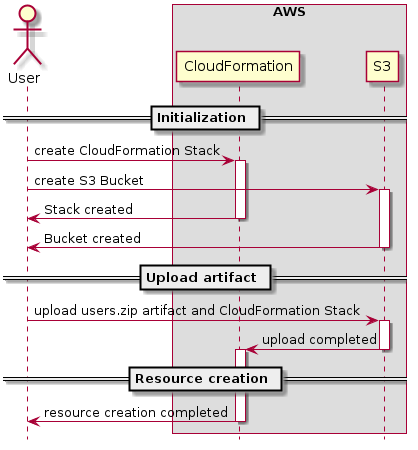
\includegraphics[width=8cm]{source/diagrams/sls_deploy_on_aws.png}
        \caption{Resources creation on Serverless deploy for a \textit{User} service}
        \label{fig:sls_deploy_on_aws}
    \end{figure}

    \subsubsection{Lambda function invocation through an API Gateway}
    \label{subsec:lambda_invocation}

    Figure \ref{fig:simple_lambda} shows the simplest possible case of execution
    flow of an http request, handled by an API Gateway, and forwarded to the Lambda
    function mapped to the user specified endpoint path.

    \begin{figure}
        \centering
        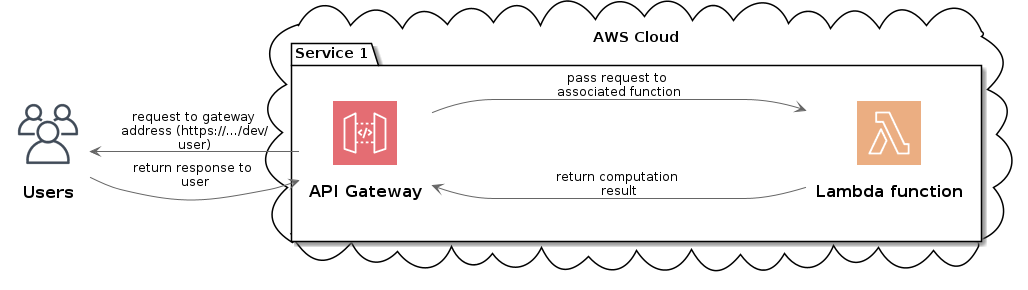
\includegraphics[width=\linewidth]{source/diagrams/lambda_invocation.png}
        \caption{Simple Lambda function execution through an API Gateway}
        \label{fig:simple_lambda}
    \end{figure}

    A more complex case is given when implementing user Authentication and hence
    restricting Lambda execution. The Authentication process is made simple by
    delegating the operation of granting or denying Authentication to a Lambda
    function, called Lambda Authorizer \cite{aws_api_gateway_doc}, as shown on
    figure \ref{fig:lambda_with_auth}. There can be two types of Lambda Authorizers:
    \begin{itemize}
        \item TOKEN: the Lambda receives the caller's identity in a bearer token.
        \item REQUEST: the Lambda receives the caller's identity in a combination
            of headers and query string parameters.
    \end{itemize}

    \begin{figure}
        \centering
        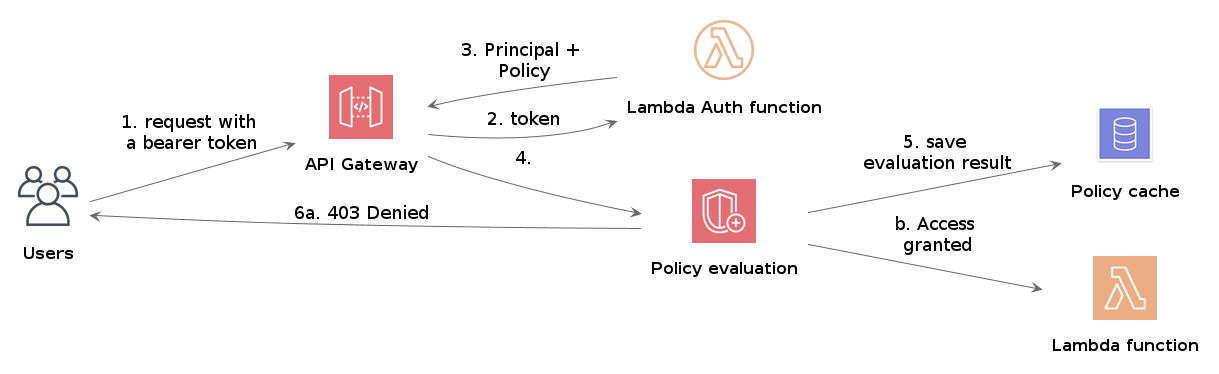
\includegraphics[width=\linewidth]{source/diagrams/lambda_authorizer.png}
        \caption{Lambda Authorizer function, based on TOKEN identity}
        \label{fig:lambda_with_auth}
    \end{figure}

    The API Gateway forward the request to the specified Lambda Authorizer, that
    checks the caller's identity and generates an Authentication Policy, which is
    an object that states which resources the user is authorized to access.
    The Policy is then cached to improve performance on subsequent requests, and
    if it the access request is granted, the flow proceed as in the previously
    described case.

    Serverless abstract this structure by allowing to specify a function as
    Authorizer of another function, as shown on listing \ref{lst:sls_auth}, where
    the \textit{getUsers} function is executed only if the function \textit{auth}
    grants access.

    \bigskip
    \begin{code}[caption=Authorizer definition on Serverless, label={lst:sls_auth},
        language=yaml]
functions:
  auth:
    handler: auth.customAuth  # auth.js
  getUsers:
    handler: users.getUsers   # users.js
    events:
      - http:
        path: hello
        method: get
        authorizer: auth
    \end{code}

    \section{React}
    An important part of the Restlessness framework is its Graphical User Interface,
    which is the main interaction point for the user. The Frontend development,
    specifically toward Web Interfaces, can count on the presence of several
    libraries and frameworks based on the JavaScript language. For the development
    of Restlessness it has been chosed the popular library React, due to its simplicity,
    and effectiveness.

    React is an Open Source JavaScript library that implements the concept of
    virtual DOM (Document Object Model) \cite{dom_standard}. The browser creates
    a DOM object at page loading, and then each Html object inside the DOM can be
    manipulated using JavaScript functions, giving the user an immediate feedback.
    React instead adopt a different approach by creating a virtual DOM alongside
    the real one. The virtual DOM is not directly synched with the real one, so
    it can be modified much faster, not having to reflect those modification on
    the screen. After those virtual DOM updates are created using the React api,
    the new istance of the virtual DOM is compared to the previous one, allowing
    to reflect the update on the real DOM only for the elements that actually
    change. The library allows to create a structure based on reusable component,
    obtaining a scalable structure, and is particularly suited for SPA (Single
    Page Applications) \cite{react_js}.
    The library also introduced a new syntax, named JSX (JavaScript XML), and
    listing \ref{lst:react_example} show the definition of a React component.

    \bigskip
    \begin{code}[caption= React component definition,label={lst:react_example}]
import React from 'react';

const Card = ({name}) => {
  return (
      <div>{name}</div>
  );
};
    \end{code}

\end{chapter}
        \begin{chapter}{Restlessness}
    \label{chap:restlessness}

    \begin{figure}
        \centering
        
\includegraphics[width=5cm]{source/images/restlessness_logo.png}
        \caption{The Restlessness logo}
    \end{figure}

    % Framework vs Library
    % Frameworks and libraries are both code written by someone else that helps you
    % perform some common tasks in a less verbose way.
    % A framework inverts the control of the program. It tells the developer what
    % they need. A library doesn’t. The programmer calls the library where and when
    % they need it.

    The Open Source framework named Restlessness was born with the goal of improving
    the developer experience of the Serverless framework, by addressing its encountered
    problems (\ref{subsec:sls_disadvantage}).
    The framework is composed by a Command Line Interface and a frontend application
    with an associated web server running locally.
    In particular the main functionalities that the framework aims to provide are:
    \begin{itemize}
        \item Creation of a new project, through the CLI, based on the typescript
            language, with a standard structure and based on the functionalities
            already offered by the Serverless framework.
        \item A local Web Interface that allows creating and managing project resources,
            functions, with their associated events and models.
        \item The creation of a standard unit testing structure for each function,
            and based on the \href{https://www.npmjs.com/package/jest}{jest} library.
        \item A standard validation structure for function's input, based on the
            \href{https://www.npmjs.com/package/yup}{yup} library.
        \item Deploy of multiple services with a single CLI command, to deal with
            the resource threshold limitation of Aws and to manage and structure
            the created project following a micro services approach.
        \item Possibility to extends the framework functionalities.
    \end{itemize}
    By addressing those points the framework aims to give developers the tools to
    focus on writing business code rather than spend time on boundary problems,
    that are important, but there may be the risk of solving the same problems
    multiple times (reinventing the wheel), which may be avoided.

    Restlessness is composed by different modular components, listed here:
    \begin{itemize}
        \item Restlessness core: core package of the framework, it contains all the
            classes and functions that provides the framework functionalities. It is
            available as \mbox{\textit{@restlessness/core}} package on npm.
        \item Command Line Interface: together with the Web Interface, this is the
            main component with which users interact the most. It depends on the
            core package to provide its functionalities and it is available as
            the \mbox{\textit{@restlessness/cli}} package on npm.
        \item Restlessness backend: api service running locally, created with the
            Restlessness framework itself. It is used by the Web Interface to
            provides its functionalities.
        \item Restlessness frontend: Web Interface with which it is possible to
            create resources and manage the project. It is part of the CLI.
    \end{itemize}
    \begin{figure}
        \centering
        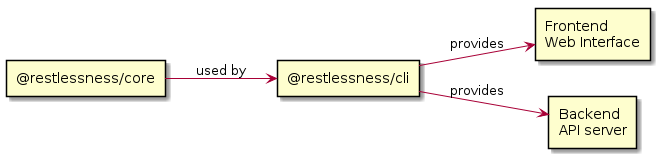
\includegraphics[width=\linewidth]{source/diagrams/rln_components.png}
        \caption{Restlessness main components}
    \end{figure}

    \section{Core}
    The core package contains the core logic components of the framework, which
    are: creation and management of resources, code generation based on templates,
    and handling of defined functions execution.
    The main resources that can be created are:
    \begin{itemize}
        \item Endpoints: endpoints are Serverless functions, triggered by and http
            event, as shown on \ref{subsec:lambda_invocation}.
        \item Schedules: schedules are Serverless functions, triggered by a
            programmed event, such as a cron job or a rate event, which is an
            event that is fired up periodically, based on the time interval provided.
        \item Authorizers: extension packages, providing Authorizer functions, as
            defined on \ref{subsec:lambda_invocation}.
        \item Daos: extensions packages, providing Data Access Object functionalities.
        \item Models: classes modeling resources, such as a User saved into a database.
            They can be associated to a Dao package, which provides its own model
            creation template.
        \item Envs: environment files, used to store information in key/value format,
            from both the user and the framework with its extensions.
        \item Services: Serverless services (i.e. \textit{serverless.json}).
    \end{itemize}

    The framework allows the creation of those resources and needs to save that
    information to be able to remember the project state, so it creates a series
    of configuration files, one for each resource type and store them under the
    \textit{config/} directory, in JSON format \cite{json_iso}.
    It has been decided to format all configuration files across the project using JSON,
    preferring it to alternatives, such as Yaml, to simplify their handling and modification
    by the framework, given that Typescript handle JSON files and objects natively.
    Given the similar structure between those files, a single abstract class models
    it, while subclasses implement specific behaviors, following the structure
    shown in figure \ref{fig:rln_json_config_file}. Each file entry has a type
    extending the interface \mbox{\textit{JsonConfigEntry}}, which contains an entry
    identifier. This structure is achieved using the Typescript feature called
    \textit{Generic Types}
    \cite{ts_generics}.

    \begin{figure}
        \centering
        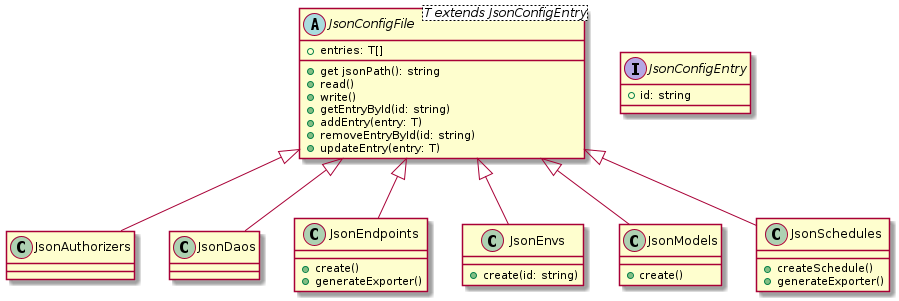
\includegraphics[width=\linewidth]{source/diagrams/rln_config_files.png}
        \caption{Configuration file classes structure}
        \label{fig:rln_json_config_file}.
    \end{figure}

    Resources created through Restlessness need to find a correspondence on the
    Serverless configuration file (\textit{serverless.yml} or \textit{serverless.json}).
    Moreover it has been decided to let the framework manages more than one service at
    a time associated to the same application or project, due to a platform limitation,
    as described on \ref{subsec:application_micro_services}.
    The structure adopted by the framework is to save the configuration file of
    each service under the \textit{serverless-services} folder and to provide by
    default two services, as shown on figure \ref{fig:sls_services_dir}.
    The first service is called \textit{shared} and is reserved for the definition
    of resources that are common across the entire application, avoiding duplicates.
    Any AWS resource can be shared and there is one in particular that's important
    to share, the API Gateway. Indeed as shown on \ref{subsec:lambda_invocation}
    Serverless automatically creates a gateway and so an api address, for each
    service and this can become cumbersome when dealing with more than one service.
    Figure \ref{fig:api_gateway_multiple_services} shows that sharing the API
    Gateway results in the user having to interact with a single endpoint.
    Other shared resources may be simple functions or authorizers.
    The other framework defined service, named \textit{offline}, is required for
    local development and it contains the resource definition of all services,
    that will be read from the serverless-offline plugin, as described on
    \ref{sec:local_dev}. Restlessness manages the synchronization between
    \textit{offline} and other user defined services transparently for the user,
    and this is one of the task of the \textit{JsonServices} class.

    \begin{figure}
        \begin{minipage}{\linewidth}
            \dirtree{%
                .1 ./.
                .2 serverless-services/.
                .3 offline.json.
                .3 shared.json.
            }
        \end{minipage}
        \caption{Services directory on a Restlessness project}
        \label{fig:sls_services_dir}
    \end{figure}

    \begin{figure}
        \centering
        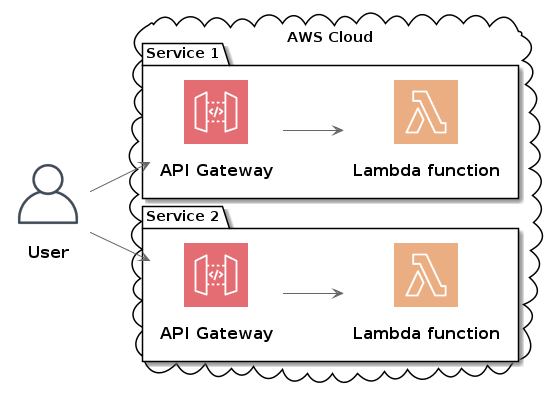
\includegraphics[width=7cm]{source/diagrams/multiple_api_gateway.png}
        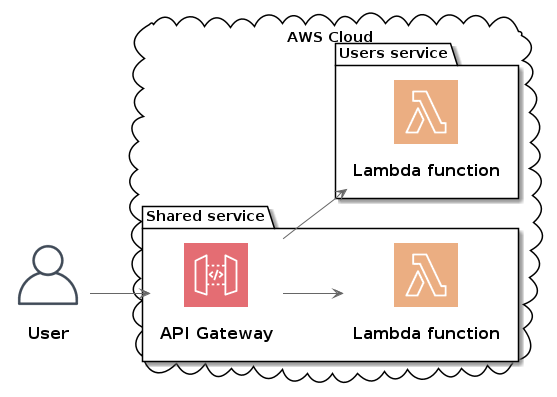
\includegraphics[width=7cm]{source/diagrams/single_api_gateway.png}
        \caption{Non shared (left) and shared (right) API Gateway on multiple services}
        \label{fig:api_gateway_multiple_services}.
    \end{figure}

    The \textit{JsonServices} class manages all operations regarding the Serverless
    services files, with the main ones being: offering CRUD methods for the various
    resources, such as: services; functions, with http or schedule events;
    serverless plugins; authorizer functions, associated to a single service or a
    shared authorizer.
    Each operation is reflected also on the \textit{offline} service.

    \subsubsection{Environment variables}
    \label{sec:env_vars}
    An important aspect when developing web applications is the handling of different
    deploying environments, as each one of them requires different configurations,
    mostly for sensitive information, such as database credentials.
    It has been decided to handle those information with different environment files,
    storing environment variables.
    When a project is created the framework generates 4 different environments: locale,
    test, staging and production. Each environment has an associated type and stage,
    with the first representing the purpose of that environment and the latter the
    corresponding Serverless stage. Below are the available types:
    \begin{itemize}
        \item test: environments used only for testing, which can happen locally
            but also through CI platform.
        \item dev: environments used for local development.
        \item deploy: environments that can be deployed.
    \end{itemize}
    All information about the environments (name, type, stage) are stored in the
    configuration file \textit{config/envs.json} and are managed by the JsonEnvs
    class.

    Environment variables are stored in the format \textit{key=value} and variable
    expansions is supported, so the value of a key can be another variable, using
    the syntax shown on listing \ref{lst:env_key_syntax}.

    \bigskip
    \begin{code}[caption=Environment variable syntax, label={lst:env_key_syntax}]
key1=${otherKey}
key2=sample ${key1}
    \end{code}

    \noindent
    Each environment is then stored under the \mbox{\textit{envs/}} directory, in
    the form \mbox{\textit{.env.<name>}} and the interaction with those files is
    handled by the \textit{EnvFile} class. The load and expansion operation is
    performed differently depending on the operation, local development or deploy.
    During local development it is the dev command that load the environment specified
    in input (\ref{sec:local_dev}). During deploy instead, the environment file
    is expanded and copied under the project root, in a file named .env, as this
    makes deploying from CI straightforward. Then at runtime the .env is automatically
    loaded by the LambdaHandler or ScheduleHandler functions.

    \subsubsection{Extensions}
    The framework has been designed from the beginning with the possibility of
    extending its functionalities using external packages.
    In order to achieve this, it has been defined an AddOnPackage class, containing
    the following lifecycle hooks:
    \begin{itemize}
        \item postInstall: executed after the addon package has been installed.
            Here it's possible to perform initialization operations.
        \item postEnvCreated: executed after a new environment has been created,
            so the addon can add its own environment variables if needed.
        \item beforeEndpoint: executed before the corresponding function of an
            endpoint. Here it's possible to perform resource initialization,
            for example opening a database connection.
        \item beforeSchedule: as for endpoints, it's executed before the
            corresponding function of a schedule.
    \end{itemize}
    In addition to this class Restlessness provides also more specific classes,
    for authentication and data access \ref{fig:rln_add_on_packages}.

    \begin{figure}
        \centering
        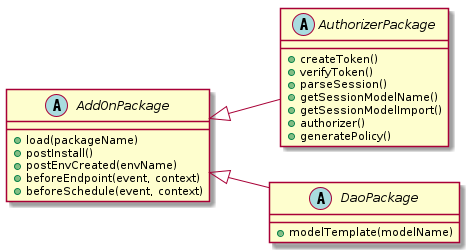
\includegraphics[width=10cm]{source/diagrams/rln_add_on_package.png}
        \caption{Add on packages structure}
        \label{fig:rln_add_on_packages}
    \end{figure}

    \subsubsection{Handlers}
    The Core package provides different functions and classes to simplify some
    operations and to provide additional functionalities on top of the Serverless
    framework.

    \paragraph{LambdaHandler} is a core function, reserved to be used for function
    associated with an http event. Its purpose is to parse the request payload and
    or query parameters, load the environment variables and execute the lifecycle
    hooks of the installed addons. After those operations the LambdaHandler executes
    the actual handler function associated for the endpoint.

    \paragraph{ScheduleHandler} behaves similarly to LambdaHandler, but it is
    reserved for functions with an associated schedule event, hence it is simpler.
    Its only tasks are to execute lifecycle hooks and the actual handler function.

    \paragraph{ResponseHandler} is a class providing static methods for generating
    response object for http endpoints. The response can be created using a JSON
    or a Buffer representation.

    \paragraph{TestHandler} is a class that simplify testing endpoints. Its main
    methods are: \textit{beforeAll}, \textit{afterAll} and \textit{invokeLambda}.
    The beforeAll function performs initialization operations, such as loading the
    correct environment variables and then the function invokeLambda executes the
    endpoint function providing automatically the event and context objects,
    simulating this way an http event. Then the afterAll function performs cleanup
    operations.
    The fact that serverless is based on function makes possible to use this simple
    testing structure, as it's not necessary for example to actually starts an http
    server to test the endpoints.

    \section{Cli}
    The Cli package provides a series of commands, listed here.

    \paragraph{new}
    Creates a new project in the current working directory, or on the specified
    input parameter.

    \paragraph{dev}
    \label{dev_command}
    The local development requires the presence of different processes, which are:
    the Api service and the Web Interface provided by Restlessness and also the
    project's process, to be able to test in real time the defined functions. The
    CLI handles those 3 processes through the dev command. In particular, both the
    project's process and Restlessness backend, are executed using the Serverless plugin
    \href{https://www.npmjs.com/package/serverless-offline}{serverless-offline},
    which allows simulating an api gateway, effectively creating a local http server.
    Instead for the frontend process it has been used the npm package
    \href{https://www.npmjs.com/package/serve}{serve}, through which is possible
    to create an http server that serves static files.
    Furthermore, the dev command takes care of executing those processes following the
    dependency order, which is: Restlessness backend, frontend and finally the
    project's process.
    Another task of the dev command is to implement inter process communication between
    itself and the backend process. This is necessary as when resources are created,
    for example endpoints or schedules, the corresponding files need to be compiled by
    typescript and also the serverless-offline plugin needs to be restarted for those
    resources to be available from the http server.
    The command receives the environment name in input, as it takes charge of loading
    the corresponding environment variables from the folder .envs, as explained on
    section \ref{sec:env_vars}. Among all environment variables, there is one, named
    \mbox{\textit{RLN\_PROJECT\_PATH}}, set by the \textit{dev} command, that indicates
    to the Backend process the path to the Restlessness project to manage.
    \begin{figure}
        \centering
        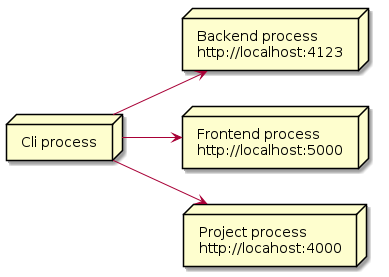
\includegraphics[width=7.5cm]{source/diagrams/rln_dev_processes.png}
        \caption{Processes generated by the dev command}
    \end{figure}

    \paragraph{create-env}
    Generates the \textit{.env} file, under project's root, corresponding to the
    environment name received as input.

    \paragraph{add-dao}
    Add an addon package of type Dao to the project, executing lifecycle hooks.

    \paragraph{add-auth}
    Add an addon package of type Auth to the project, executing lifecycle hooks.

    \paragraph{deploy}
    The Serverless Framework already provides a command for the deploy operation,
    as shown on \ref{sec:serverless_framework}, however with the micro services
    oriented structure suggested by Restlessness this operation is more elaborated,
    as it involves the deploy of more than one service, in a particular order.
    This is necessary because of the presence of the \textit{shared} resources
    service, so to successfully deploy a service that uses resources from the
    \textit{shared} one, it is necessary that those resources already exist.
    The correct deploy ordering is then \textit{shared} service first, followed
    by all the other services.
    It should be noted that the \textit{offline} service is not involved in the
    deploy process as it's used only for local development.
    To address this operations the Restlessness CLI provides a custom deploy
    command (listing \ref{lst:rln_command_deploy}).

    \bigskip
    \begin{code}[caption=Deploy command, label={lst:rln_command_deploy}, language=shell]
$ restlessness deploy
$ restlessness deploy --env production
$ restlessness deploy --env production users
    \end{code}

    It is possible to deploy the application on different environments, otherwise
    the command assume staging as the default environment.
    It is also possible to perform the deploy of just a single service, to keep
    the whole development, test and deploy process fast and easy, when making small
    changes, in accordance with the serverless paradigm.
    Since the deploy operation involves more than one service, it's important that
    the information among them are consistent, especially when deploying. This is
    why the deploy command, under the hood, takes care of performing this check,
    with a method from the \textit{JsonServices} class, named \textit{healthCheck}.
    In particular, it checks that the various services belong to the same serverless
    organization and organization, the same AWS deploy region and that do not exist
    services with functions associated to the same path. The latter is due to the fact
    that the services use a shared api gateway.

    \paragraph{remove}
    Complementary command with respect to \textit{deploy}, it removes all services
    enforcing an opposite ordering doing so.

    \subsubsection{Backend}
    The Restlessness backend provides the endpoints used by the frontend to show,
    create, update and delete the framework resources described previously.
    It has been created with the Restlessness framework itself and it relies on
    the \mbox{\textit{@restlessness/core}} package to provide its functionalities.
    It is run locally using the
    \href{https://www.npmjs.com/package/serverless-offline}{serverless-offline}
    plugin, resulting in a lightweight Api Service.
    The Restlessness resources that the Api provides coincide with the resources
    already described, which are: Endpoints, Schedules, Authorizers, Daos, Envs,
    Models and Services.
    For each resource it has been created a corresponding Model, to map the information
    received from the core package into the format expected by the frontend and
    vice versa. All Models inherit basic functionalities from a base class named
    \textit{BaseModel} (\ref{fig:base_model_class}), with utility methods for
    accessing data and the unimplemented methods \textit{toConfigEntry} and
    \textit{fromConfigEntry}, that perform map operations.
    Figure \ref{fig:backend_endpoint_flow} shows the flow for a request regarding
    the creation of an endpoint.

    \begin{figure}
        \centering
        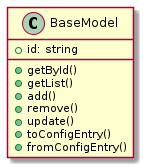
\includegraphics[width=3cm]{source/diagrams/rln_backend_base_model.png}
        \caption{BaseModel class}
        \label{fig:base_model_class}
    \end{figure}

    \begin{figure}
        \centering
        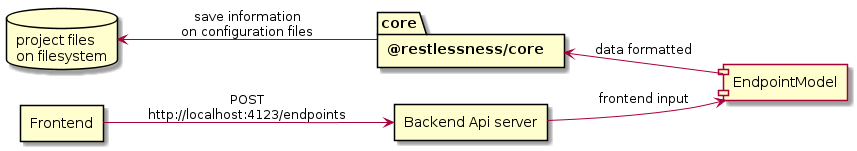
\includegraphics[width=\linewidth]{source/diagrams/rln_backend_endpoint_creation.png}
        \caption{Creation of an endpoint}
        \label{fig:backend_endpoint_flow}
    \end{figure}

    \subsubsection{Frontend}
    The Restlessness frontend provides a simple interface to interact with the
    framework. Once opened a dashboard provides some project's information and
    links to pages for each resource, where it is possible to view the current
    resources create and modify them.
    Figure \ref{fig:frontend_site_map} shows the site map of the frontend.

    \begin{figure}
        \centering
        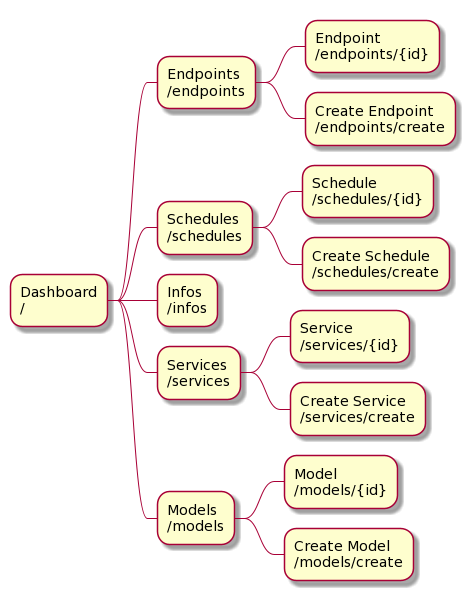
\includegraphics[width=8cm]{source/diagrams/frontend_site_map.png}
        \caption{Restlessness frontend site map}
        \label{fig:frontend_site_map}
    \end{figure}

    \section{Usage}
    \label{sec:rln_project_usage}

    The Restlessness CLI is available for installation on the npm platform. Once
    installed, the first step toward using the framework is the creation of a new
    project and that is possible using the \textit{new} command, as shown
    on listing \ref{lst:rln_command_new}.

    \bigskip
    \begin{code}[caption=New command, label={lst:rln_command_new}, language=shell]
$ restlessness new rln_project
    \end{code}

    Once the command has finished, a new folder has been created, with a completely
    structured restlessness project, as can be see in figure
    \ref{fig:sample_rln_project_folder}.

    \begin{figure}
        \begin{minipage}{\linewidth}
            \dirtree{%
                .1 ./.
                .2 .restlessness.json.
                .2 configs/.
                .3 authorizers.json.
                .3 daos.json.
                .3 default-headers.json.
                .3 endpoints.json.
                .3 envs.json.
                .3 models.json.
                .3 schedules.json.
                .2 envs/.
                .3 .env.locale.
                .3 .env.production.
                .3 .env.staging.
                .3 .env.test.
                .2 serverless-services/.
                .3 offline.json.
                .3 shared.json.
                .2 src/.
                .3 exporter.ts.
                .3 schedulesExporter.ts.
            }
        \end{minipage}
        \caption{Sample Restlessness project structure}
        \label{fig:sample_rln_project_folder}
    \end{figure}

    The sample project shown in figure \ref{fig:sample_rln_project_folder} however,
    does not include all generated files, as some of them are not strictly part of
    the framework, but are required from other used tools, in particular:
    \begin{itemize}
        \item .eslintrc.json: configuration file of the linter
            \href{https://eslint.org/}{eslint}.
        \item .gitignore: it lists intentionally ignored files from the git tracking
            system.
        \item package.json: entry point of every npm project, it lists the project
            dependencies, as well as other project related information, such as
            the project name and version.
        \item package-lock.json: npm generated file, it contains a snapshot of the
            version of all dependencies, with the goal of obtaining reproducible
            builds.
        \item tsconfig.json: configuration file for the Typescript compiler.
    \end{itemize}

    The first noticeable difference with respect to a plain serverless project is the
    lack of a serverless.yml (or serverless.json) file under the root, instead it
    is present the \textit{serverless-services/} directory with the default services
    \textit{shared} and \textit{offline}.
    Other created files are: configuration files, under the \textit{config} folder,
    environment files, source code, under the src folder and a .restlessness.json
    file, used to store project related information needed by the framework.

    \subsection{Local development}
    \label{sec:local_dev}

    The \textit{dev} command starts the processes as described on \ref{dev_command},
    producing the output shown on \ref{lst:rln_command_dev}.

    \bigskip
    \begin{code}[caption=Dev command, label={lst:rln_command_dev}, language=shell]
$ restlessness dev locale
$ RESTLESSNESS: Running on http://localhost:5000
$ rln-project: offline: Starting Offline: dev/us-east-1.
$ rln-project: offline: Offline listening on http://local...
$            * clean: rln-project-offline-dev-clean
$ rln-project:
$       POST | http://localhost:4000/dev/users
    \end{code}

    \subsection{Resource creation}
    The Web Interface looks like in the figure \ref{fig:rln_web_interface} and
    provides some project details, such as serverless organization, application
    (section \ref{sec:serverless_framework}) and finally the aws data center
    region to which the project will be deployed.
    The main functionalities are then available through some shortcuts, that allow
    creating and consulting resources, such as endpoints, schedules, services and
    models.

    \begin{figure}
        \centering
        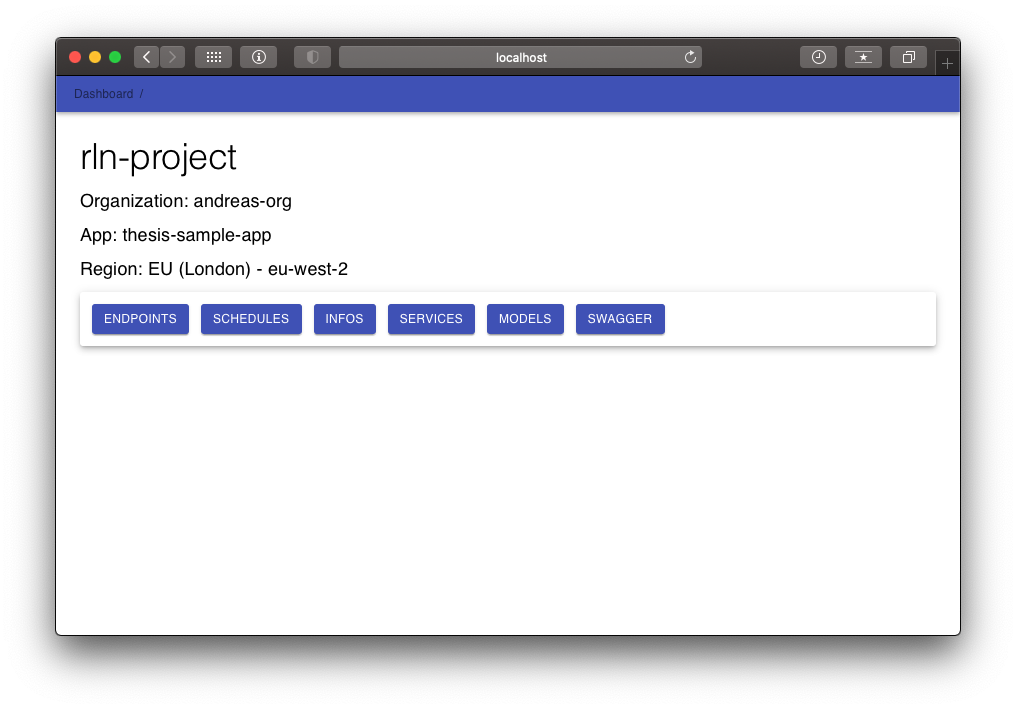
\includegraphics[width=\linewidth]{source/images/rln-web-interface.png}
        \caption{Restlessness Web Interface}
        \label{fig:rln_web_interface}
    \end{figure}

    Being Restlessness a framework for serverless services, the primary resource
    that can be defined are functions and at the moment it is possible to define
    two type of functions, based on the event that triggers them. They are endpoints,
    and schedules.

    \subsubsection{Endpoints}
    \label{subsec:endpoints}
    It is possible to create an endpoint from the Web Interface, by specifying the
    following fields, as shown on figure \ref{fig:wi_create_endpoint}:
    \begin{itemize}
        \item Service: the service to which the function must be associated.
        \item Route: the path corresponding to the serverless function.
        \item Method: the http method.
        \item Warmup enabled: enable or disable the warmup plugin
            (\ref{subsec:cold_start})
        \item Daos: Associated Data Access Object addon.
        \item Authorizer: this optional field sets a further function, that
            perform the authorization operation, granting or denying access to
            the specified function.
    \end{itemize}

    \begin{figure}
        \centering
        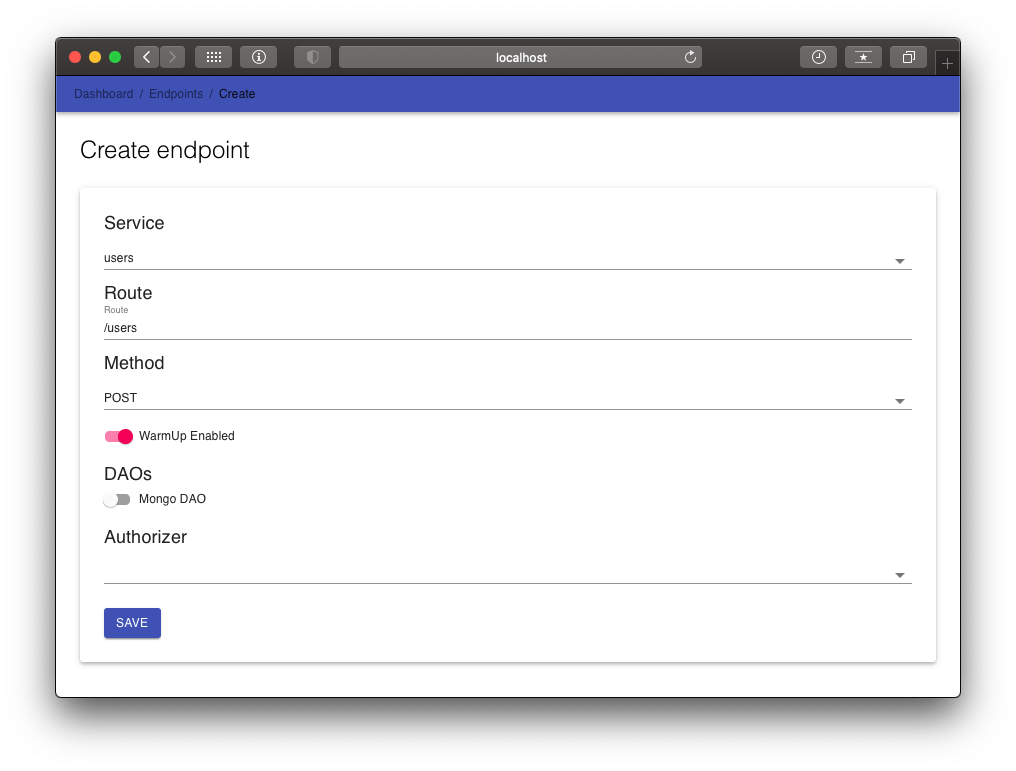
\includegraphics[width=\linewidth]{source/images/rln-wi-create-endpoint.png}
        \caption{Creation of and endpoint}
        \label{fig:wi_create_endpoint}
    \end{figure}

    During the endpoint creation, the framework takes care of saving the provided
    information on the configuration file \textit{config/endpoints.json} and to
    create code template for the development of the corresponding function.
    As shown on figure \ref{fig:new_endpoint_folder_structure}, it has been created a
    folder under src/endpoints, using the notation http method plus normalized value
    of the http path.

    \begin{figure}
        \begin{minipage}{\linewidth}
            \dirtree{%
                .1 ./.
                .2 src/.
                .3 endpoints/.
                .4 post-users.
                .5 handler.ts.
                .5 index.ts.
                .5 index.test.ts.
                .5 interfaces.ts.
                .5 validations.ts.
                .3 exporter.ts.
                .3 schedulesExporter.ts.
            }
        \end{minipage}
        \caption{Structure of a new endpoint folder}
        \label{fig:new_endpoint_folder_structure}
    \end{figure}

    The developer can then code the function on the \textit{handler.ts} file, which
    already contains a template (listing \ref{lst:handler_ts}) and define the
    validation object in \textit{validations.ts} (listing \ref{lst:validations_ts}).
    It is also possible to exploit the Typescript functionalities, defining the various
    interface for the request, response and query parameters objects, all under the
    interfaces.ts file (listing \ref{lst:interfaces_ts}).
    The actual function entry point that will be executed once deployed is defined
    in the file \textit{index.ts} (listing \ref{lst:index_ts}). This function is
    created binding the function LambdaHandler input with the handler function and
    validation object.

    \clearpage

    \begin{code}[caption=handler.ts content, label={lst:handler_ts}]
export default async (req: Request) => {
  try {
    const {
        validationResult,
        payload,
    } = req;

    if (!validationResult.isValid) {
        return ResponseHandler.json({
            message: validationResult.message
        }, StatusCodes.BadRequest);
    }

    return ResponseHandler.json({});
  } catch (e) {
    console.error(e);
    return ResponseHandler.json(
        {}, StatusCodes.InternalServerError);
  }
};
    \end{code}

    \bigskip
    \begin{code}[caption=index.ts content, label={lst:index_ts}]
export default LambdaHandler
    .bind(this, handler, validations, 'postUsers');
    \end{code}

    \bigskip
    \begin{code}[caption=validations.ts content, label={lst:validations_ts}]
const queryStringParametersValidations =
  (): YupShapeByInterface<QueryStringParameters>  => ({});

const payloadValidations =
  (): YupShapeByInterface<Payload> => ({});

export default () => ({
  queryStringParameters: yup.object()
    .shape(queryStringParametersValidations()),
  payload: yup.object()
    .shape(payloadValidations()).noUnknown(),
});
    \end{code}

    \bigskip
    \begin{code}[caption=interfaces.ts content, label={lst:interfaces_ts}]
import { RequestI } from '@restlessness/core';
export interface QueryStringParameters {}
export interface Payload {}
export interface Request extends
    RequestI<QueryStringParameters, Payload, null> {};
    \end{code}

    \subsubsection{Schedules}
    \label{subsec:schedules}
    Schedules are serverless functions that are triggered by a programmed event.
    By creating a Schedule from the Web Interface the framework creates the necessary
    template files under \textit{src/schedules} as shown on
    \ref{fig:new_schedule_folder_structure} and also saves the provided information
    under the \textit{config/schedules.json} file.

    \begin{figure}
        \begin{minipage}{\linewidth}
            \dirtree{%
                .1 ./.
                .2 src/.
                .3 schedules/.
                .4 clean/.
                .5 handler.ts.
                .5 index.ts.
            }
        \end{minipage}
        \caption{Structure of a schedule endpoint folder}
        \label{fig:new_schedule_folder_structure}
    \end{figure}

    The structure of the template files is similar to the one generated for endpoints,
    but simpler. The \textit{handler.ts} file contains the function that the developer
    has to code, while the \textit{index.ts} file is the entry point.
    The core function ScheduleHandler is used to wrap the handler function, the same
    way as happens for endpoints, with the purpose of executing the framework lifecycle
    hooks.

    \bigskip
    \begin{code}[caption=handler.ts content, label={lst:sched_handler_ts}]
export default async (event) => {};
    \end{code}

    \bigskip
    \begin{code}[caption=index.ts content, label={lst:sched_index_ts}]
import { ScheduleHandler } from '@restlessness/core';
import handler from './handler';
export default ScheduleHandler.bind(this, handler, 'clean');
    \end{code}

    \subsection{Test}
    A test template is also provided when creating a new endpoint and it is based
    on the popular unit testing library \href{https://jestjs.io/}{jest}, in
    conjunction with the TestHandler class provided by Restlessness.

    \bigskip
    \begin{code}[caption=index.test.ts template, label={lst:endopints_test_ts}]
const postUsers = 'postUsers';

beforeAll(async done => {
  await TestHandler.beforeAll();
  done();
});

describe('postUsers API', () => {
  test('', async (done) => {
    const res = await TestHandler.invokeLambda(
        postUsers);
    // expect(res.statusCode).toBe(StatusCodes.OK);
    done();
  });
});

afterAll(async done => {
  await TestHandler.afterAll();
  done();
});
    \end{code}

\end{chapter}
        \begin{chapter}{Restlessness Extensions}
    \label{chap:extensions}

    \section{Authorization}
    Serverless functions can also perform authorization operations, as described
    on \ref{subsec:lambda_invocation}. Restlessness provides the abstract class
    \textit{AuthorizerPackage}, extending \textit{AddOnPackage}, which provides
    a standard structure to define token based authorizer functions.

    \begin{figure}
        \centering
        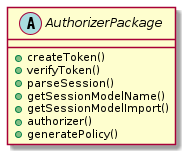
\includegraphics[width=5.5cm]{source/diagrams/authorizer_package_class.png}
        \caption{AuthorizerPackage class}
    \end{figure}

    \subsection{Jwt Authorizer}
    Restlessness already provides the package \mbox{\textit{@restlessness/auth-jwt}},
    implementing the Json Web Token authorization method, defined as:

    \enquote*{%
        JSON Web Token (JWT) is an open standard (RFC 7519) that defines a compact
        and self-contained way for securely transmitting information between parties
        as a JSON object. This information can be verified and trusted because it
        is digitally signed. JWTs can be signed using a secret (with the HMAC
        algorithm) or a public/private key pair using RSA or ECDSA.%
    } \cite{json_web_token}

    \noindent
    In its compact form, the token consist of three parts separated by dots,
    which are:
    \begin{itemize}
        \item Header: It typically consists of two parts: the type of token, which
            is \textit{JWT} and the signing algorithm used. The JSON object
            containing those keys is then Base64url encoded, creating the first
            part of the token.
        \item Payload: It contains the claims, which are statements about an entity,
            which usually is the user, plus any additional data. Also this JSON
            object is then Base64url encoded and it forms the second part of the token.
        \item Signature: The third part is the signature obtained by signing the
            already created parts (Header and Payload separated by a dot) with a
            secret.
    \end{itemize}
    The final output is composed by three Base64url strings, separated by dots,
    that can be easily passed in an Http environment. In the case of the Jwt
    Authorizer function it will be included in the requests in the
    \textit{Authorization} header, with type \textit{Bearer}.

    \subsection{Usage example}
    The package can be used on a Restlessness project following this steps:

    \paragraph{Installation}
    The package can be installed using the npm CLI and then added to the project
    using the Restlessness CLI, particularly with the \textit{add-auth} command
    (\ref{lst:auth_jwt_install}).

    \bigskip
    \begin{code}[caption=auth-jwt installation, label={lst:auth_jwt_install},  language=shell]
$ npm install @restlessness/auth-jwt
$ restlessness add-auth @restlessness/auth-jwt
    \end{code}

    \paragraph{Model creation}
    Once installed, the package automatically creates a model class, named
    \textit{JwtSession}, based on the template defined by the package and it can
    then be extended as needed (\ref{lst:new_model_auth}).

    \bigskip
    \begin{code}[caption=A JwtSession class created by the auth-jwt package, label={lst:new_model_auth}]
export default class JwtSession {
  ['constructor']: typeof JwtSession
  id: string

  async serialize(): Promise<string> {
    return JSON.stringify(this);
  }

  static async deserialize(
      session: string): Promise<JwtSession> {
    const jwtSession = new JwtSession();
    Object.assign(jwtSession, JSON.parse(session));
    return jwtSession;
  }
};
    \end{code}

    \paragraph{Model usage}
    It's then possible to create a session and generate the Jwt token, as shown
    on \ref{lst:jwt_usage}.

    \bigskip
    \begin{code}[caption=User model usage, label={lst:jwt_usage}]
// Generate session and serialize it
const session = new JwtSession();
session.id = myId;
session.name = 'Arthur';
session.permissions = [];
// Once serialized, the session can be
// easily returned to the user
const serialized = session.serialize();

// Deserialize the session
const deserialized = JwtSession.deserialize(serialized);
console.log(deserialized.name) // --> Output: Arthur
    \end{code}

    \section{Data Access Object}
    \label{sec:data_access_object}

    To simplify the creation of a Data Access Object, Restlessness provides the
    abstract class \textit{DaoPackage} (listing \ref{lst:daopackage}), which extends
    the \textit{AddOnPackage} class previously defined.

    \bigskip
    \begin{code}[caption=DaoPackage class definition, label={lst:daopackage}]
abstract class DaoPackage extends AddOnPackage {
    abstract modelTemplate(modelName: string): string
}
    \end{code}

    In addition to the previously defined hooks, classes implementing DaoPackage,
    should implement also the modelTemplate method and a base dao class, to which
    we will refer to as DaoBase. This latter class should provides the main Dao
    functionalities, while the code template returned by modelTemplate should define
    a class that extends the DaoBase one.

    \subsection{Dao for mongodb}
    Restlessness already provides a Dao package for the popular non relational
    database \href{https://www.mongodb.com/}{mongodb} and it's available on the
    npm platform as \mbox{\textit{@restlessness/dao-mongo}}.
    That package exports two main components: an implementation of the DaoPackage
    class and a MongoBase class, the base class containing the main Dao
    functionalities for CRUD operations, as shown on listing \ref{fig:mongobase}.

    \begin{figure}
        \centering
        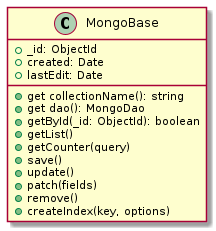
\includegraphics[width=5.5cm]{source/diagrams/mongobase_class.png}
        \caption{MongoBase class}
        \label{fig:mongobase}
    \end{figure}

    Users of the package can then create models based on the MongoBase class through
    the Restlessness Web Interface.
    The creation of that model is made possible by implementing the
    \textit{DaoPackage.modelTemplate} method, as shown on listing \ref{lst:model_template}.

    \bigskip
    \begin{code}[caption=modelTemplate function definition, label={lst:model_template}]
const modelTemplate = (name: string): string => `
import {
    MongoBase, ObjectId
} from '@restlessness/dao-mongo';

export default class ${name} extends MongoBase {
    ['constructor']: typeof ${name}

    static get collectionName() {
        return '${pluralize(name, 2).toLowerCase()}';
    }
};
`;
    \end{code}

    \subsubsection{Database Proxy}
    \label{subsec:database_proxy}
    The MongoBase class uses the MongoDao class internally to perform database
    operations. The latter class, at the early stage of Restlessness development,
    offered an abstraction layer over the official
    \href{https://www.npmjs.com/package/mongodb}{mongodb driver} for Node.js,
    effectively using the driver internally.
    As described on chapter \ref{chap:application}, this approach showed its
    drawbacks in the context of a serverless application, so the next approach has
    been to exploit the concept of Database Proxy.
    The main idea is to have a serverless function, the proxy, with the task of
    performing all database access, on behalf of all other serverless functions.
    Another advantage of Serverless is indeed the possibility to invoke a function
    from another one, but this comes at the cost of a doubled Cold start (
    \ref{subsec:cold_start}), resulting in a performance degradation for some requests.
    However, the solution provided on \ref{subsec:cold_start} is particularly useful in
    this case because enabling the warmup plugin on the proxy function, avoids the
    costs of function initialization and also database connection, making it possible
    to enable warmup only on a small group of functions, so the overall performance
    improves or stays the same.

    \begin{figure}
        \centering
        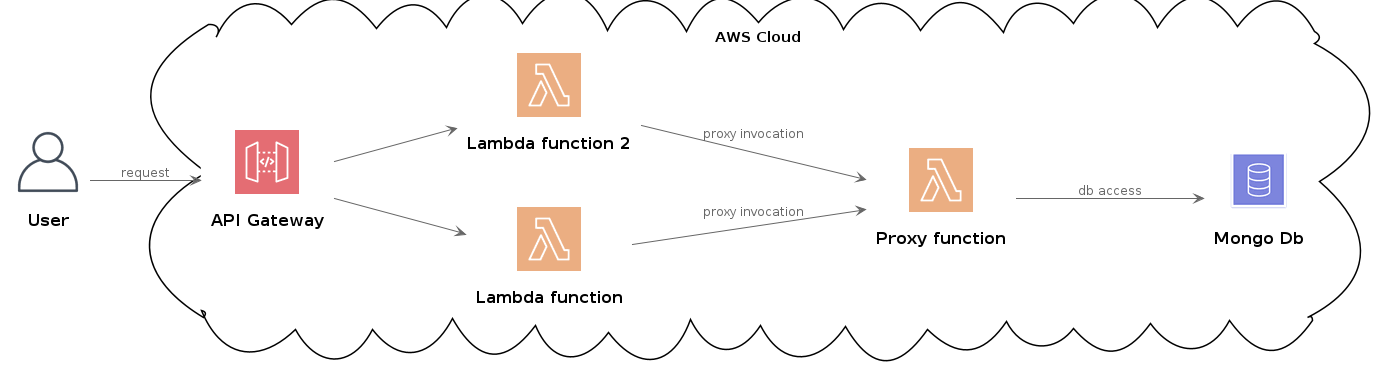
\includegraphics[width=\linewidth]{source/diagrams/mongo_proxy.png}
        \caption{Mongo proxy structure}
    \end{figure}

    To implement this structure it has been developed a serverless plugin, named
    \href{https://www.npmjs.com/package/serverless-mongo-proxy}{serverless-mongo-proxy}
    and usable independently of the Restlessness framework.
    The plugin automatically creates the serverless proxy function in the specified
    service, which in the case of Restlessness is the shared one, so all services
    can exploit the advantages of using a proxy.
    Since all information exchanged between serverless functions must be serialized,
    the plugin used the \href{http://bsonspec.org/}{bson} encoding, to obtain consistent
    representation for data types such as dates and regular expressions.

    The MongoDao class can then invoke the proxy function internally, without having
    to keep a connection open.

    \subsection{Usage example}
    The package can be used on a Restlessness project following this steps:

    \paragraph{Installation}
    It is possible to install the package using the npm CLI and then adding it to
    the enabled restlessness addons using the restlessness CLI command \textit{add-dao}
    (\ref{lst:dao_mongo_install}).

    \bigskip
    \begin{code}[caption=dao-mongo installation, label={lst:dao_mongo_install}, language=shell]
$ npm install @restlessness/dao-mongo
$ restlessness add-dao @restlessness/dao-mongo
    \end{code}

    \paragraph{Model creation}
    Once installed it is possible to create, from the Web Interface, models based on
    the Dao class provided by the package (\ref{fig:wi_dao_mongo_model}).

    This corresponds to the creation of a model template that can be extended with
    methods and fields (\ref{lst:new_model})

    \bigskip
    \begin{code}[caption=A new model based on the dao-mongo package, label={lst:new_model}]
export default class User extends MongoBase {
  ['constructor']: typeof User
  name: string
  age: number

  static get collectionName() {
    return 'users';
  }
};
    \end{code}

    \paragraph{Model usage}
    It's then possible to perform database operations, exploiting the abstraction
    provided by the MongoBase class, as shown on \ref{lst:user_model_usage}.

    \bigskip
    \begin{code}[caption=User model usage, label={lst:user_model_usage}]
const user = new User();
user.name = 'Andrea';
user.age = 25;
await user.save();
    \end{code}

    \begin{figure}
        \centering
        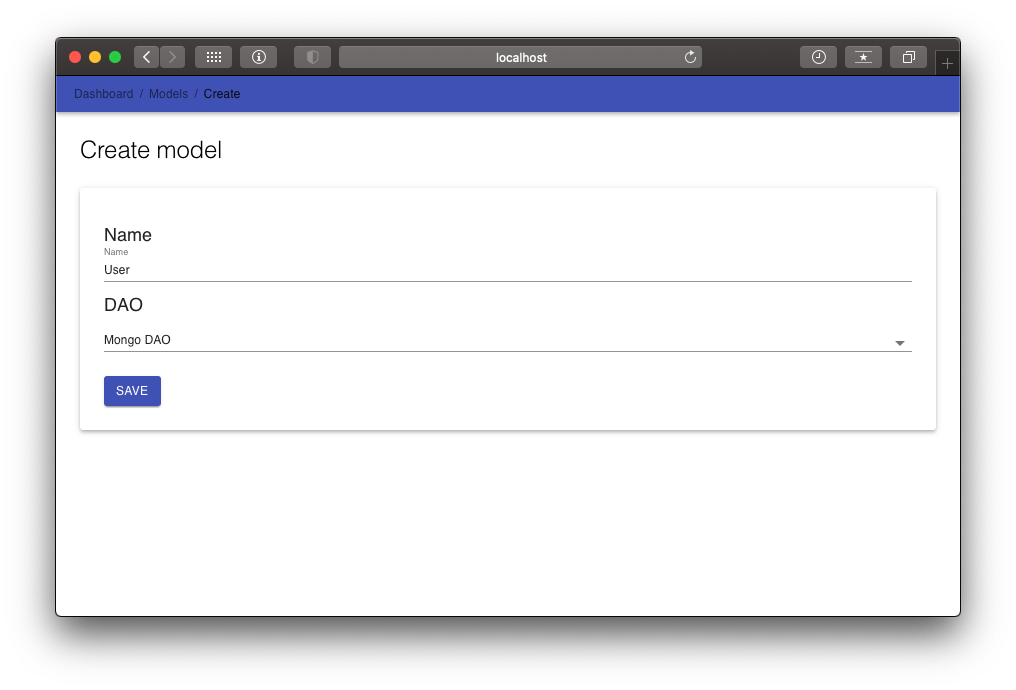
\includegraphics[width=\linewidth]{source/images/rln-wi-create-model.png}
        \caption{Creation of a Model}
        \label{fig:wi_dao_mongo_model}
    \end{figure}

\end{chapter}
        \begin{chapter}{Application}
    \label{chap:application}

    During its development process, the Restlessness framework has been tested on
    real deployed applications, and this has been fundamental as it helped finding
    bugs and critical issues at an early stage.
    The main issues have emerged during the implementation of the backend for the
    project Spazio alla scuola, a platform thought by the Fondazione Agnelli.

    The foundation is a non-profit, independent institute for social science research,
    born in 1966 in Turin, by the lawyer Agnelli, on the occasion of the centenary
    of the birth of the founder of Fiat, Senator Giovanni Agnelli.
    Its purpose is to work in support of scientific research and to disseminate
    knowledge of the conditions on which Italy's progress depends.

    The project Spazio alla scuola aims to provide a concrete support to school
    leaders for lecture resumption on September 2020, given the health situation on the
    country due to the SARS-CoV-2 pandemic.
    The platform offer tools to verify capacity of classroom and other school spaces,
    to plan classrooms flows and staggering, in compliance with the distancing measures.
    The platform is provided as a free service and is available at the address
    \url{www.spazioallascuola.it}.

    \section{Cold start}
    \label{subsec:cold_start}

    The first encountered problem has been Cold start, a new term in the serverless
    development that denotes the situation in which a serverless function is not
    active yet, so the platform must perform some resources initialization, with the
    main one being\footnote{Relatively to the Aws platform}:

    \begin{itemize}
        \item Code: the project's code is uploaded in a zip archive, so it needs to
            be downloaded and extracted.
        \item Extensions: aws allow associate extensions to a lambda function, to
            integrate it with custom monitoring, security or other tools.
        \item Runtime: bootstrap operation for the chosen runtime environment,
            it is also possible to provides a custom runtime if needed.
        \item Function: code written by the developer, it can perform some resource
            initialization, such as creating a database connection.
    \end{itemize}

    \begin{figure}
        \centering
        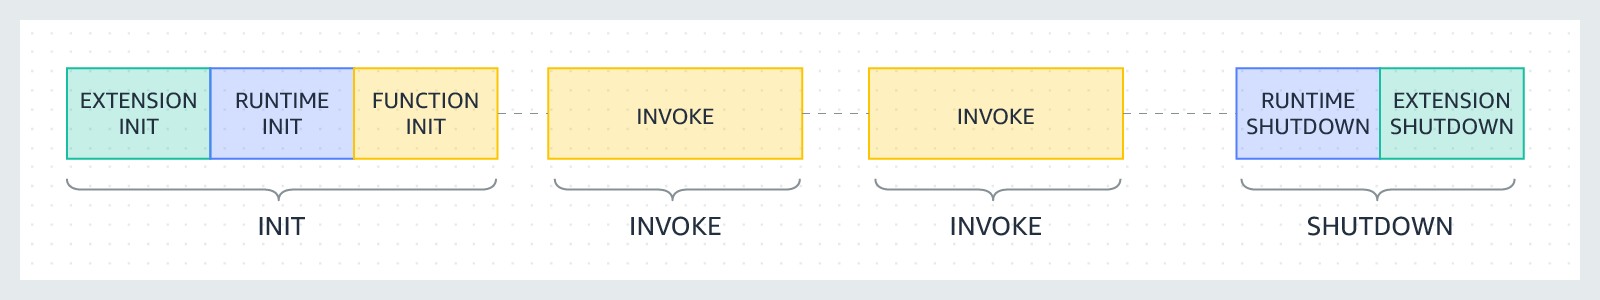
\includegraphics[width=\linewidth]{source/images/aws-lambda-lifecycle.png}
        \caption{Aws Lambda lifecycle}
        \label{fig:aws_lambda_lifecycle}
    \end{figure}

    The Cold start refers exactly to this Init phase and represent an overhead to the
    function execution, however once this phase is completed the function is ready,
    and subsequent invocations will not suffer from it. Then after some times without
    receiving any events, usually in the order of 5 to 20 minutes, the platform performs
    the Shutdown phase, so any following event causes the process to start again from
    the Init phase.
    For the majority of runtimes the duration of the Cold start varies in the order
    of tenths of a second, as shown on figure \ref{fig:cold_start_duration}. The provided
    numbers vary also based on the memory allocated for the function and the size of the
    provided code package.

    \begin{figure}
        \centering
        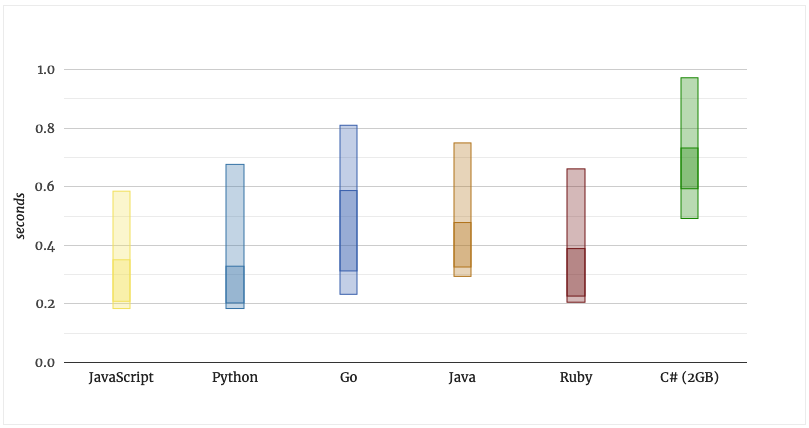
\includegraphics[width=\linewidth]{source/images/cold-start-duration.png}
        \caption{Cold start duration for different runtimes}
        \label{fig:cold_start_duration}
    \end{figure}

    In the particular case of the project Spazio alla scuola the Cold start duration
    was experienced to be in the order of 1.5s, caused mainly from: mongodb
    initialization and connection (about 500ms) and third party libraries (about 400ms)
    and Restlessness overhead (about 50ms).

    One of the approaches to mitigate the effect of the Cold start proposed by the
    Serverless community has been the plugin named
    \href{https://www.npmjs.com/package/serverless-plugin-warmup}{serverless-plugin-warmup}.
    The plugin creates a scheduled function programmed to invoke the other defined functions,
    forcing the platform to keep an active container for each function.
    This way the Cold start effect remains present, but the end user of the api does
    not experience it.

    It as been decided to make this plugin an integral part of the Restlessness framework,
    granting out of the box support for it. From the Web Interface is possible to
    enabled or disable the warmup on the single endpoint, since not all functions may
    need it.
    By including the warmup plugin into the framework the effect of Cold start has
    been mitigated, however it introduced another type of issue.

    \section{Database proxy}
    The project Spazio alla scuola rely on the popular non relational database
    \href{https://www.mongodb.com}{mongodb}. As stated previously, each function
    run in its own runtime, independently from the others, consequently each function
    requiring database access needs to open a non shared connection.
    So the number of active connections can become quite high, depending on the number
    of active functions, furthermore using mongodb, the connection remains active for
    a certain amount of time even after the function has been shutdown.
    This leads to a high number of active connections, which is a problem, not only
    in terms of resources used, since each connection requires memory usage on the
    database, but also because mongodb has a limit of 500 concurrent connections,
    and once the threshold is exceeded the application experiences random errors when
    performing database operations.
    \begin{figure}
        \centering
        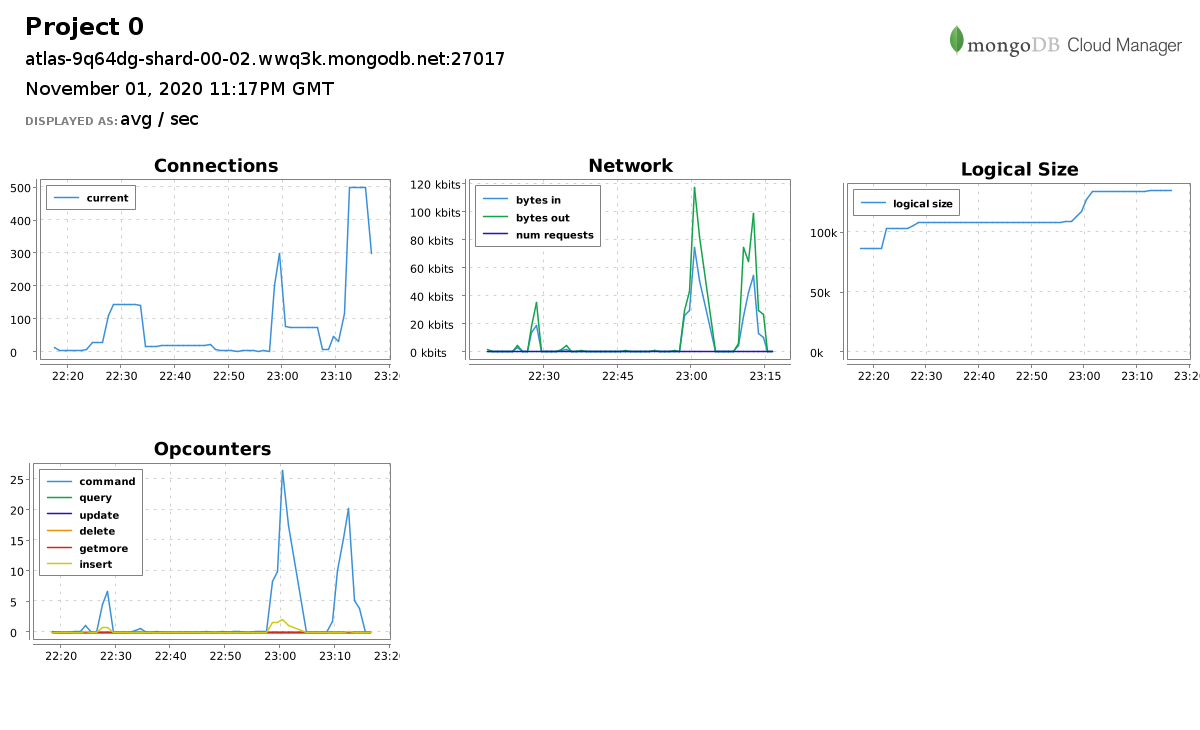
\includegraphics[width=7cm]{source/images/mongo-connections.png}
        \caption{Mongodb connections reaching the 500 threshold}
    \end{figure}

    Although the problem has been amplified by the introduction of the warmup plugin
    integration, it remains a critical issue for application that rely on the high
    scalability of the serverless platform.
    To address this problem on its relational databases, Aws rely on the usage of a
    proxy between the functions and the database. Exploiting the concept of a proxy,
    has been decided to approach the problem in the same way, since a solution for
    for the mongo database does not exist at the moment.
    Restlessness already provides the package @restlessness/dao-mongo, as described on
    section \ref{sec:data_access_object}, defining an abstraction level over the
    mongodb driver, so it was possible to include a proxy without changing the
    exposed methods for the users.
    Has been decided to develop an open source plugin, named
    \href{https://github.com/getapper/serverless-mongo-proxy}{serverless-mongo-proxy},
    to provide the proxy functionality, independently from the Restlessness framework,
    as shown on \ref{subsec:database_proxy}.
    The dao-mongo package then uses the plugin internally, providing an effective
    solution to the presented problem.

    \section{Micro services}
    \label{subsec:application_micro_services}
    During the deployment of an application on the Aws platform a number of resources
    are created for each function, to provides services such as logging, api gateway
    for http events, permissions and others functionalities. The Aws platform has a
    threshold of maximum 200 resources definable for each service
    (\ref{subsec:sls_disadvantage}), and since for each function there are about 10
    resources associated, it follows that each service can define about 20 functions.
    Since the serverless paradigm proposes a Micro services oriented approach this
    limitation actually force developers to compose their application as a set of
    low complexity services.
    So the next step in the Restlessness framework development has been to switch
    between the management of a single service, to a multitude of services, under
    the same Restlessness project. With this approach has been possible to split
    the functions of the project Spazio alla scuola into multiple services, obtaining
    a more fine grained separation between its logic components.

    \bigbreak
    In conclusion the choice of using serverless, combined with the Restlessness
    framework for the backend api of Spazio alla scuola, brought the desired benefits
    in terms of ease of development, after the proper framework improvements described
    previously. At its peak, the api service has managed 500 thousand requests,
    demonstrating the advantage of the natural scalability of the serverless approach.

\end{chapter}

        \begin{chapter}{Future Works}

    At the end of this development cycle, Restlessness can be defined as production
    ready, being used on real deployed app successfully.
    However its development is not completed, and on its roadmap there are a series
    of features and improvements to do. While at the moment the framework supports
    only the AWS cloud providers, one of the main objectives is to make the framework
    effectively platform agnostic, thus providing support for other providers, firstly
    for Google Cloud Platform and Microsoft Azure Functions. This feature represents
    a great challenge, as each provider's platform must be studied in its details
    to being able to offer the same functionalities cross platforms.

    Regarding code testing there is a structure for unit testing, but at the moment
    there is no proposed solution for integration testing. In this case, it will be
    possible to create a lightweight structure exploiting the fact that serverless
    is based on functions, as it has been done for unit testing.

    Another planned improvement is to bring all Cli functionalities on the Web
    Interface, and vice versa, giving developers more flexibility when it comes
    to manage a Restlessness based project.

    Last but not least, the list of provided extensions can be increased, by
    supporting other databases or authentication methods.

\end{chapter}
        \begin{thebibliography}{9}

    \bibitem{sls_paradigm} What is serverless
    \url{https://www.cloudflare.com/learning/serverless/what-is-serverless}

    \bibitem{iaas} What is IaaS
    \url{https://www.cloudflare.com/learning/cloud/what-is-iaas}

    \bibitem{paas} What is PaaS
    \url{https://www.cloudflare.com/learning/serverless/glossary/platform-as-a-service-paas}

    \bibitem{saas} What is SaaS
    \url{https://www.cloudflare.com/learning/cloud/what-is-saas}

    \bibitem{sls_pro_cons} Serverless pros and cons
    \url{https://hackernoon.com/what-is-serverless-architecture-what-are-its-pros-and-cons-cc4b804022e9}

    \bibitem{sls_aws_doc} Serverless Framework Aws Guide
    \url{https://www.serverless.com/framework/docs/providers/aws/guide/intro}

    \bibitem{separation_of_concerns}  Dijkstra, Edsger W (1982).
    "On the role of scientific thought". Selected writings on Computing: A Personal
    Perspective. New York, NY, USA: Springer-Verlag. pp. 60–66. ISBN 0-387-90652-5.
    \url{https://www.cs.utexas.edu/users/EWD/transcriptions/EWD04xx/EWD447.html}

    \bibitem{data_access_object} Data Access Object Pattern
    \url{https://www.oracle.com/java/technologies/dataaccessobject.html}

    \bibitem{spazio_alla_scuola} Spazio alla scuola
    \url{https://www.fondazioneagnelli.it/2020/07/17/spazio-alla-scuola}

    \bibitem{aws_doc_runtimes} Aws Lambda Environment
    \url{https://docs.aws.amazon.com/lambda/latest/dg/runtimes-context.html}

\end{thebibliography}

    \end{mainmatter}

\end{document}
